% A list of all figure files:
% Those produced by TraubMemorial.m
%	f1f2plot.eps
%	f1closeplot.eps
%	f1ppf2ppplot.eps
%	f2closeplot.eps
%	f3plot.eps
%	f3ppplot.eps
%	sampling-funappxg.eps
%	f3foolplot.eps
%	sampling-funming.eps

%
%	chebfun_errors.eps
%	funappx_g_errors.eps
%	traub_funappxNoPenalty_g_test.eps
%	f4_funappx_error.eps
%	f4_funmin_g.eps


\documentclass[review]{elsarticle}
%\documentclass[final]{elsarticle}

\usepackage{amsmath,amssymb,amsthm,xspace,mathtools,hyperref,color}
\usepackage{mathrsfs,verbatim,xspace}

\allowdisplaybreaks
\newcommand{\bvec}[1]{\boldsymbol{#1}}
%\newcommand{\bvec}[1]{\text{\boldmath$#1$}}
\newcommand{\avec}[1]{\vec{#1}}
%\renewcommand{\vec}[1] {\text{\boldmath$#1$}}
%\renewcommand{\vec}[1]{\ensuremath{\mathbf{#1}}}
\newcommand{\vecsym}[1]{\ensuremath{\boldsymbol{#1}}}
\def\bbl{\text{\boldmath$\{$}}
\def\bbr{\text{\boldmath$\}$}}
\newcommand{\bbrace}[1]{\bbl #1 \bbr}
\newcommand{\bbbrace}[1]{\mathopen{\pmb{\bigg\{}}#1\mathclose{\pmb{\bigg\}}}}
%\def\bbl{\boldsymbol{\left \{}}
%\def\bbr{\boldsymbol{\right \}}}
\def\betahat{\hat\beta}
%\def\e{\text{e}}
%\def\E{\text{E}}
\newcommand{\dif}{{\rm d}}

\newlength{\overwdth}
\def\overstrike#1{ 
\settowidth{\overwdth}{#1}\makebox[0pt][l]{\rule[0.5ex]{\overwdth}{0.1ex}}#1}

\def\abs#1{\ensuremath{\left \lvert #1 \right \rvert}}
\newcommand{\bigabs}[1]{\ensuremath{\bigl \lvert #1 \bigr \rvert}}
\newcommand{\Bigabs}[1]{\ensuremath{\Bigl \lvert #1 \Bigr \rvert}}
\newcommand{\biggabs}[1]{\ensuremath{\biggl \lvert #1 \biggr \rvert}}
\newcommand{\Biggabs}[1]{\ensuremath{\Biggl \lvert #1 \Biggr \rvert}}
\newcommand{\norm}[2][{}]{\ensuremath{\left \lVert #2 \right \rVert}_{#1}}
\newcommand{\bignorm}[2][{}]{\ensuremath{\bigl \lVert #2 \bigr \rVert}_{#1}}
\newcommand{\Bignorm}[2][{}]{\ensuremath{\Bigl \lVert #2 \Bigr \rVert}_{#1}}
\newcommand{\biggnorm}[2][{}]{\ensuremath{\biggl \lVert #2 \biggr \rVert}_{#1}}
\newcommand{\ip}[3][{}]{\ensuremath{\left \langle #2, #3 \right \rangle_{#1}}}

\newcommand{\bigvecpar}[3]{\ensuremath{\bigl ( #1 \bigr )_{#2}^{#3}}}
\newcommand{\Bigvecpar}[3]{\ensuremath{\Bigl ( #1 \Bigr )_{#2}^{#3}}}
\newcommand{\biggvecpar}[3]{\ensuremath{\biggl ( #1 \biggr )_{#2}^{#3}}}
\newcommand{\bigpar}[1]{\ensuremath{\bigl ( #1 \bigr )}}
\newcommand{\Bigpar}[1]{\ensuremath{\Bigl ( #1 \Bigr )}}
\newcommand{\biggpar}[1]{\ensuremath{\biggl ( #1 \biggr )}}

\newcommand{\IIDsim}{\overset{\textup{IID}}{\sim}}

\DeclareMathOperator{\success}{succ}
\DeclareMathOperator{\sinc}{sinc}
\DeclareMathOperator{\sech}{sech}
\DeclareMathOperator{\csch}{csch}
\DeclareMathOperator{\dist}{dist}
\DeclareMathOperator{\spn}{span}
\DeclareMathOperator{\sgn}{sgn}
\DeclareMathOperator*{\rmse}{rmse}
\DeclareMathOperator{\Prob}{\mathbb{P}}
\DeclareMathOperator{\Ex}{\mathbb{E}}
\DeclareMathOperator{\rank}{rank}
\DeclareMathOperator{\erfc}{erfc}
\DeclareMathOperator{\erf}{erf}
\DeclareMathOperator{\cov}{cov}
\DeclareMathOperator{\cost}{cost}
\DeclareMathOperator{\comp}{comp}
\DeclareMathOperator{\corr}{corr}
\DeclareMathOperator{\diag}{diag}
\DeclareMathOperator{\var}{var}
\DeclareMathOperator{\opt}{opt}
\DeclareMathOperator{\brandnew}{new}
\DeclareMathOperator{\std}{std}
\DeclareMathOperator{\kurt}{kurt}
\DeclareMathOperator{\med}{med}
\DeclareMathOperator{\vol}{vol}
\DeclareMathOperator{\bias}{bias}
\DeclareMathOperator*{\argmin}{argmin}
\DeclareMathOperator{\sign}{sign}
\DeclareMathOperator{\spann}{span}
\DeclareMathOperator{\cond}{cond}
\DeclareMathOperator{\trace}{trace}
\DeclareMathOperator{\Si}{Si}
%\DeclareMathOperator{\diag}{diag}
\DeclareMathOperator{\col}{col}
\DeclareMathOperator{\nullspace}{null}
\DeclareMathOperator{\Order}{{\mathcal O}}
%\DeclareMathOperator{\rank}{rank}

\newcommand{\vzero}{\bvec{0}}
\newcommand{\vone}{\bvec{1}}
\newcommand{\vinf}{\bvec{\infty}}
\newcommand{\va}{\bvec{a}}
\newcommand{\vA}{\bvec{A}}
\newcommand{\vb}{\bvec{b}}
\newcommand{\vB}{\bvec{B}}
\newcommand{\vc}{\bvec{c}}
\newcommand{\vd}{\bvec{d}}
\newcommand{\vD}{\bvec{D}}
\newcommand{\ve}{\bvec{e}}
\newcommand{\vf}{\bvec{f}}
\newcommand{\vF}{\bvec{F}}
\newcommand{\vg}{\bvec{g}}
\newcommand{\vG}{\bvec{G}}
\newcommand{\vh}{\bvec{h}}
\newcommand{\vi}{\bvec{i}}
\newcommand{\vj}{\bvec{j}}
\newcommand{\vk}{\bvec{k}}
\newcommand{\vl}{\bvec{l}}
\newcommand{\vell}{\bvec{\ell}}
\newcommand{\vL}{\bvec{L}}
\newcommand{\vm}{\bvec{m}}
\newcommand{\vp}{\bvec{p}}
\newcommand{\vq}{\bvec{q}}
\newcommand{\vr}{\bvec{r}}
\newcommand{\vs}{\bvec{s}}
\newcommand{\vS}{\bvec{S}}
\newcommand{\vt}{\bvec{t}}
\newcommand{\vT}{\bvec{T}}
\newcommand{\vu}{\bvec{u}}
\newcommand{\vU}{\bvec{U}}
\newcommand{\vv}{\bvec{v}}
\newcommand{\vV}{\bvec{V}}
\newcommand{\vw}{\bvec{w}}
\newcommand{\vW}{\bvec{W}}
\newcommand{\vx}{\bvec{x}}
\newcommand{\vX}{\bvec{X}}
\newcommand{\vy}{\bvec{y}}
\newcommand{\vY}{\bvec{Y}}
\newcommand{\vz}{\bvec{z}}
\newcommand{\vZ}{\bvec{Z}}

\newcommand{\ai}{\avec{\imath}}
\newcommand{\ak}{\avec{k}}
\newcommand{\avi}{\avec{\bvec{\imath}}}
\newcommand{\at}{\avec{t}}
\newcommand{\avt}{\avec{\vt}}
\newcommand{\ax}{\avec{x}}
\newcommand{\ah}{\avec{h}}
\newcommand{\akappa}{\avec{\kappa}}
\newcommand{\avx}{\avec{\vx}}
\newcommand{\ay}{\avec{y}}
\newcommand{\avy}{\avec{\vy}}
\newcommand{\avz}{\avec{\vz}}
\newcommand{\avzero}{\avec{\vzero}}
\newcommand{\aomega}{\avec{\omega}}
\newcommand{\avomega}{\avec{\vomega}}
\newcommand{\anu}{\avec{\nu}}
\newcommand{\avnu}{\avec{\vnu}}
\newcommand{\aDelta}{\avec{\Delta}}
\newcommand{\avDelta}{\avec{\vDelta}}

\newcommand{\valpha}{\bvec{\alpha}}
\newcommand{\vbeta}{\bvec{\beta}}
\newcommand{\vgamma}{\bvec{\gamma}}
\newcommand{\vdelta}{\bvec{\delta}}
\newcommand{\vDelta}{\bvec{\Delta}}
\newcommand{\vphi}{\bvec{\phi}}
\newcommand{\vvphi}{\bvec{\varphi}}
\newcommand{\vomega}{\bvec{\omega}}
\newcommand{\vlambda}{\bvec{\lambda}}
\newcommand{\vmu}{\bvec{\mu}}
\newcommand{\vnu}{\bvec{\nu}}
\newcommand{\vpsi}{\bvec{\psi}}
\newcommand{\vepsilon}{\bvec{\epsilon}}
\newcommand{\veps}{\bvec{\varepsilon}}
\newcommand{\veta}{\bvec{\eta}}
\newcommand{\vxi}{\bvec{\xi}}
\newcommand{\vtheta}{\bvec{\theta}}
\newcommand{\vtau}{\bvec{\tau}}
\newcommand{\vzeta}{\bvec{\zeta}}

\newcommand{\hvb}{\hat{\vb}}
\newcommand{\hcc}{\widehat{\cc}}
\newcommand{\hD}{\widehat{D}}
\newcommand{\hE}{\widehat{E}}
\newcommand{\hf}{\widehat{f}}
\newcommand{\hF}{\widehat{F}}
\newcommand{\hg}{\hat{g}}
\newcommand{\hvf}{\widehat{\bvec{f}}}
\newcommand{\hh}{\hat{h}}
\newcommand{\hH}{\widehat{H}}
\newcommand{\hi}{\hat{\imath}}
\newcommand{\hI}{\hat{I}}
\newcommand{\hci}{\widehat{\ci}}
\newcommand{\hj}{\hat{\jmath}}
\newcommand{\hp}{\hat{p}}
\newcommand{\hP}{\hat{P}}
\newcommand{\hS}{\widehat{S}}
\newcommand{\hv}{\hat{v}}
\newcommand{\hV}{\widehat{V}}
\newcommand{\hx}{\hat{x}}
\newcommand{\hX}{\widehat{X}}
\newcommand{\hvX}{\widehat{\vX}}
\newcommand{\hy}{\hat{y}}
\newcommand{\hvy}{\hat{\vy}}
\newcommand{\hY}{\widehat{Y}}
\newcommand{\hvY}{\widehat{\vY}}
\newcommand{\hZ}{\widehat{Z}}
\newcommand{\hvZ}{\widehat{\vZ}}

\newcommand{\halpha}{\hat{\alpha}}
\newcommand{\hvalpha}{\hat{\valpha}}
\newcommand{\hbeta}{\hat{\beta}}
\newcommand{\hvbeta}{\hat{\vbeta}}
\newcommand{\hgamma}{\hat{\gamma}}
\newcommand{\hvgamma}{\hat{\vgamma}}
\newcommand{\hdelta}{\hat{\delta}}
\newcommand{\hvareps}{\hat{\varepsilon}}
\newcommand{\hveps}{\hat{\veps}}
\newcommand{\hmu}{\hat{\mu}}
\newcommand{\hnu}{\hat{\nu}}
\newcommand{\hvnu}{\widehat{\vnu}}
\newcommand{\homega}{\widehat{\omega}}
\newcommand{\hrho}{\hat{\rho}}
\newcommand{\hsigma}{\hat{\sigma}}
\newcommand{\htheta}{\hat{\theta}}
\newcommand{\hTheta}{\hat{\Theta}}
\newcommand{\htau}{\hat{\tau}}
\newcommand{\hxi}{\hat{\xi}}
\newcommand{\hvxi}{\hat{\vxi}}

\newcommand{\otau}{\overline{\tau}}
\newcommand{\oY}{\overline{Y}}

\newcommand{\rD}{\mathring{D}}
\newcommand{\rf}{\mathring{f}}
\newcommand{\rV}{\mathring{V}}

\newcommand{\ta}{\tilde{a}}
\newcommand{\tA}{\tilde{A}}
\newcommand{\tmA}{\widetilde{\mA}}
\newcommand{\tvb}{\tilde{\vb}}
\newcommand{\tcb}{\widetilde{\cb}}
\newcommand{\tB}{\widetilde{B}}
\newcommand{\tc}{\tilde{c}}
\newcommand{\tvc}{\tilde{\vc}}
\newcommand{\tfc}{\tilde{\fc}}
\newcommand{\tC}{\widetilde{C}}
\newcommand{\tcc}{\widetilde{\cc}}
\newcommand{\tD}{\widetilde{D}}
\newcommand{\te}{\tilde{e}}
\newcommand{\tE}{\widetilde{E}}
\newcommand{\tf}{\widetilde{f}}
\newcommand{\tF}{\widetilde{F}}
\newcommand{\tvf}{\tilde{\vf}}
\newcommand{\tcf}{\widetilde{\cf}}
\newcommand{\tg}{\tilde{g}}
\newcommand{\tG}{\widetilde{G}}
\newcommand{\tildeh}{\tilde{h}}
\newcommand{\tH}{\widetilde{H}}
\newcommand{\tch}{\widetilde{\ch}}
\newcommand{\tK}{\widetilde{K}}
\newcommand{\tvk}{\tilde{\vk}}
\newcommand{\tM}{\widetilde{M}}
\newcommand{\tn}{\tilde{n}}
\newcommand{\tN}{\widetilde{N}}
\newcommand{\tQ}{\widetilde{Q}}
\newcommand{\tR}{\widetilde{R}}
\newcommand{\tS}{\widetilde{S}}
\newcommand{\tvS}{\widetilde{\vS}}
\newcommand{\tT}{\widetilde{T}}
\newcommand{\tv}{\tilde{v}}
\newcommand{\tV}{\widetilde{V}}
\newcommand{\tvx}{\tilde{\vx}}
\newcommand{\tW}{\widetilde{W}}
\newcommand{\tx}{\tilde{x}}
\newcommand{\tX}{\widetilde{X}}
\newcommand{\tvX}{\widetilde{\vX}}
\newcommand{\ty}{\tilde{y}}
\newcommand{\tvy}{\tilde{\vy}}
\newcommand{\tz}{\tilde{z}}
\newcommand{\tZ}{\widetilde{Z}}
\newcommand{\tL}{\tilde{L}}
\newcommand{\tP}{\widetilde{P}}
\newcommand{\tY}{\widetilde{Y}}
\newcommand{\tmH}{\widetilde{\mH}}
\newcommand{\tmK}{\widetilde{\mK}}
\newcommand{\tmM}{\widetilde{\mM}}
\newcommand{\tmQ}{\widetilde{\mQ}}
\newcommand{\tct}{\widetilde{\ct}}
\newcommand{\talpha}{\tilde{\alpha}}
\newcommand{\tdelta}{\tilde{\delta}}
\newcommand{\tDelta}{\tilde{\Delta}}
\newcommand{\tvareps}{\tilde{\varepsilon}}
\newcommand{\tveps}{\tilde{\veps}}
\newcommand{\tlambda}{\tilde{\lambda}}
\newcommand{\tmu}{\tilde{\mu}}
\newcommand{\tnu}{\tilde{\nu}}
\newcommand{\trho}{\tilde{\rho}}
\newcommand{\tvarrho}{\tilde{\varrho}}
\newcommand{\ttheta}{\tilde{\theta}}
\newcommand{\tsigma}{\tilde{\sigma}}
\newcommand{\tvmu}{\tilde{\vmu}}
\newcommand{\tphi}{\tilde{\phi}}
\newcommand{\tPhi}{\widetilde{\Phi}}
\newcommand{\tvphi}{\tilde{\vphi}}
\newcommand{\ttau}{\tilde{\tau}}
\newcommand{\txi}{\tilde{\xi}}
\newcommand{\tvxi}{\tilde{\vxi}}


\newcommand{\mA}{\mathsf{A}}
\newcommand{\mB}{\mathsf{B}}
\newcommand{\mC}{\mathsf{C}}
\newcommand{\vmC}{\bvec{\mC}}
\newcommand{\mD}{\mathsf{D}}
\newcommand{\mF}{\mathsf{F}}
\newcommand{\mG}{\mathsf{G}}
\newcommand{\mH}{\mathsf{H}}
\newcommand{\mI}{\mathsf{I}}
\newcommand{\mK}{\mathsf{K}}
\newcommand{\mL}{\mathsf{L}}
\newcommand{\mM}{\mathsf{M}}
\newcommand{\mP}{\mathsf{P}}
\newcommand{\mQ}{\mathsf{Q}}
\newcommand{\mR}{\mathsf{R}}
\newcommand{\mS}{\mathsf{S}}
\newcommand{\mT}{\mathsf{T}}
\newcommand{\mU}{\mathsf{U}}
\newcommand{\mV}{\mathsf{V}}
\newcommand{\mW}{\mathsf{W}}
\newcommand{\mX}{\mathsf{X}}
\newcommand{\mLambda}{\mathsf{\Lambda}}
\newcommand{\mSigma}{\mathsf{\Sigma}}
\newcommand{\mzero}{\mathsf{0}}
\newcommand{\mGamma}{\mathsf{\Gamma}}

\newcommand{\bbE}{\mathbb{E}}
\newcommand{\bbF}{\mathbb{F}}
\newcommand{\bbK}{\mathbb{K}}
\newcommand{\bbZ}{\mathbb{Z}}
\newcommand{\bbone}{\mathbbm{1}}
\newcommand{\naturals}{\mathbb{N}}
\newcommand{\reals}{\mathbb{R}}
\newcommand{\integers}{\mathbb{Z}}
\newcommand{\natzero}{\mathbb{N}_{0}}
\newcommand{\rationals}{\mathbb{Q}}
\newcommand{\complex}{\mathbb{C}}

\newcommand{\ca}{\mathcal{A}}
\newcommand{\cb}{\mathcal{B}}
\providecommand{\cc}{\mathcal{C}}
\newcommand{\cd}{\mathcal{D}}
\newcommand{\cf}{\mathcal{F}}
\newcommand{\cg}{\mathcal{G}}
\newcommand{\ch}{\mathcal{H}}
\newcommand{\ci}{\mathcal{I}}
\newcommand{\cj}{\mathcal{J}}
\newcommand{\ck}{\mathcal{K}}
\newcommand{\cl}{\mathcal{L}}
\newcommand{\cm}{\mathcal{M}}
\newcommand{\tcm}{\widetilde{\cm}}
\newcommand{\cn}{\mathcal{N}}
\newcommand{\cp}{\mathcal{P}}
\newcommand{\calr}{\mathcal{R}}
\newcommand{\cs}{\mathcal{S}}
\newcommand{\ct}{\mathcal{T}}
\newcommand{\cu}{\mathcal{U}}
\newcommand{\cv}{\mathcal{V}}
\newcommand{\cw}{\mathcal{W}}
\newcommand{\cx}{\mathcal{X}}
\newcommand{\tcx}{\widetilde{\cx}}
\newcommand{\cy}{\mathcal{Y}}
\newcommand{\cz}{\mathcal{Z}}

\newcommand{\fc}{\mathfrak{c}}
\newcommand{\fC}{\mathfrak{C}}
\newcommand{\fh}{\mathfrak{h}}
\newcommand{\fu}{\mathfrak{u}}

\newcommand{\me}{\ensuremath{\mathrm{e}}} % for math number 'e', 2.718 281 8..., tha base of natural logarithms
\newcommand{\mi}{\ensuremath{\mathrm{i}}} % for math number 'i', the imaginary unit
\newcommand{\mpi}{\ensuremath{\mathrm{\pi}}} % for math number 'pi', the circumference of a circle of diameter 1


\journal{Journal of Complexity}

%%%%%%%%%%%%%%%%%%%%%%%
%% Elsevier bibliography styles
%%%%%%%%%%%%%%%%%%%%%%%
%% To change the style, put a % in front of the second line of the current style and
%% remove the % from the second line of the style you would like to use.
%%%%%%%%%%%%%%%%%%%%%%%

%% Numbered
\bibliographystyle{model1-num-names}

%% Numbered without titles
%\bibliographystyle{model1a-num-names}

%% Harvard
%\bibliographystyle{model2-names.bst}\biboptions{authoryear}

%% Vancouver numbered
%\usepackage{numcompress}\bibliographystyle{model3-num-names}

%% Vancouver name/year
%\usepackage{numcompress} \bibliographystyle{model4-names}\biboptions{authoryear}

%% APA style
%\bibliographystyle{model5-names}\biboptions{authoryear}

%% AMA style
%\usepackage{numcompress}\bibliographystyle{model6-num-names}

%% `Elsevier LaTeX' style
%\bibliographystyle{elsarticle-num}
%%%%%%%%%%%%%%%%%%%%%%%

\newcommand{\abstol}{\varepsilon}
%\newcommand{\abstol}{\varepsilon_{\textrm{a}}}
\newcommand{\datasites}{\{x_i\}_{i=0}^n}
\makeatletter
\newcommand{\vast}{\bBigg@{4}}
\newcommand{\Vast}{\bBigg@{6}}
\makeatother
%\newdefinition{algo}{Algorithm}
\theoremstyle{definition}
\newtheorem*{algoA}{Algorithm $A$}
\newtheorem*{algoM}{Algorithm $M$}
\newcommand{\vastl}{\mathopen\vast}
\newcommand{\vastm}{\mathrel\vast}
\newcommand{\vastr}{\mathclose\vast}
\newcommand{\Vastl}{\mathopen\Vast}
\newcommand{\Vastm}{\mathrel\Vast}
\newcommand{\Vastr}{\mathclose\Vast}
\renewcommand{\cw}{W}

\definecolor{orange}{rgb}{1.0,0.3,0.0}
\definecolor{violet}{rgb}{0.75,0,1}
\definecolor{darkgreen}{rgb}{0,0.6,0}
\newcommand{\frednote}[1]{  {\textcolor{red}  {\mbox{**Fred:} #1}}}
\newcommand{\yuhannote}[1]{  {\textcolor{darkgreen}  {\mbox{**Yuhan:} #1}}}
\newcommand{\xinnote}[1]{ {\textcolor{violet}  {\mbox{**Xin:} #1}}}
\newcommand{\scnote}[1]{ {\textcolor{orange}  {\mbox{**SC:} #1}}}

\newcommand{\Ixl}{I_{x,l}}
\newcommand{\Ixlx}{I_{x,\ell(x)}}
\newcommand{\Ixrlx}{I_{x,\rell(x)}}
\newcommand{\Ixhlx}{I_{x,\hell(x)}}
\newcommand{\hell}{\hat{\ell}}
\newcommand{\tell}{\tilde{\ell}}
\newcommand{\ttL}{\widetilde{\widetilde{L}}}
\newcommand{\chL}{\widehat{L}}
\newcommand{\rell}{\mathring{\ell}}
\newcommand{\tgamma}{\widetilde{\gamma}}
\newcommand{\hM}{\widehat{M}}
\DeclareMathOperator{\lo}{lo}
\DeclareMathOperator{\ninit}{ninit}
\DeclareMathOperator{\errest}{errest}
\newtheorem{theorem}{Theorem}
\newtheorem{exmp}{Example}
\newtheorem{prop}[theorem]{Proposition}
\newcommand{\funappxg}{\texttt{funappx\_g}\xspace}
\newcommand{\funappxglobalg}{\texttt{funappxglobal\_g\xspace}}
\newcommand{\funming}{\texttt{funmin\_g\xspace}}
\newcommand{\fminbnd}{\texttt{fminbnd\xspace}}
\newcommand{\integralg}{\texttt{integral\_g\xspace}}
\newcommand{\cosappx}{\widehat{\operatorname*{cos}}}
\newcommand{\sinappx}{\widehat{\operatorname*{sin}}}
\newcommand{\minfi}{\min\limits_{i=1, \ldots,  n} f(x_i)} %minf(xi)
\newcommand{\minfii}{\min(f(x_{i-1}), f(x_i))} %min{f(x_i-1),f(x_i)}
\begin{document}

\begin{frontmatter}

\title{Local Adaption for Approximation and Minimization of Univariate Functions}


%% Group authors per affiliation:
\author{Sou-Cheng T.~Choi}
\author{Yuhan Ding}
\author{Fred J.~Hickernell}
\address{Department of Applied Mathematics, Illinois Institute of Technology, RE 208, 10 West 32$^{\text{nd}}$ Street, Chicago, Illinois, 60616, USA}
\author{Xin Tong}
\address{Department of Mathematics, Statistics, and Computer Science, University of Illinois at Chicago, Room 322 SEO, 851 S. Morgan Street, Chicago, Illinois, 60607, USA}



\begin{abstract}
Nearly all adaptive algorithms for function approximation and minimization lack theoretical guarantees.  Our new locally adaptive algorithms are guaranteed to provide answers that satisfy a user-specified absolute error tolerance for a cone, $\cc$, of non-spiky functions in the Sobolev space $\cw^{2,\infty}$.  These algorithms automatically determine where to sample the function---sampling more densely where the second derivative is larger.  The computational cost to approximate a function with $L^{\infty}$ error no greater than $\abstol$ is essentially $\Order\Bigl(\sqrt{\norm[\frac12]{f''}/\abstol}\Bigr)$.  This is the same order as that of the best function approximation algorithm for functions in $\cc$. The computational cost of the new minimization algorithm is no worse than that for function approximation and can be much smaller if the function significantly exceeds its minimum value over much of its domain.  Our  algorithms have been implemented in our Guaranteed Automatic Integration Library.  Numerical examples are presented to illustrate the performance of our algorithms.
\end{abstract}

\begin{keyword}
adaption \sep automatic \sep computational complexity \sep function approximation \sep function recovery \sep minimization \sep optimization
\MSC[2010]  65D05 \sep 65D07 \sep 65K05 \sep 68Q25
\end{keyword}

\end{frontmatter}

%%%%%%%%%%%%%%%%%%%%%%%%%%%%%%%%%%%%%%%%%%%%%%%%%%
\section{Introduction} \label{sec:intro}
%%%%%%%%%%%%%%%%%%%%%%%%%%%%%%%%%%%%%%%%%%%%%%%%%%

The goal of this paper is to solve univariate function approximation and global minimization problems by locally adaptive algorithms. For some suitable set, $\cc$, of continuous,
real-valued functions defined on a finite interval $[a,b]$, we  construct
algorithms $A:(\cc,(0,\infty)) \to L^{\infty}[a,b]$ and $M: (\cc,(0,\infty)) \to
\reals$ such that for any $f \in \cc$ and any error tolerance $\abstol > 0$,
\begin{gather}
\norm{f - A(f,\abstol)} \le \abstol,  \tag{APP} \label{appxprob} \\
0 \le M(f,\abstol) - \min_{a \le x \le b} f(x)  \le \abstol. \tag{MIN} \label{optprob}
\end{gather}
Here, $\norm{\cdot}$ denotes the $L^{\infty}$-norm on $[a,b]$.  The algorithms $A$ and $M$ depend only on function values. These algorithms choose their data sites in the domain adaptively, with each new site depending on the function data already obtained.  Each algorithm  automatically determines when to stop sampling
and return the correct answer.  These algorithms sample more densely where needed, i.e., they are locally adaptive.

Adaptive algorithms relieve the user of having to specify the number of samples required.  Only the desired error tolerance is needed.  Existing adaptive numerical algorithms for function approximation, such as the MATLAB toolbox Chebfun \citep{TrefEtal16a}, are successful for some $f$, but fail for other $f$.  No theory explains for which $f$ Chebfun succeeds.   A corresponding situation exists for minimization algorithms, such as \texttt{min} in Chebfun or MATLAB's built-in \texttt{fminbnd} \citep{MAT9.0}.

Our aim is to provide practical algorithms for both \eqref{appxprob} and  \eqref{optprob} with theoretical justification.  Here we accomplish the following:
\begin{itemize}

\item The set $\cc$ for which our algorithms succeed is defined in Section~\ref{sec:conedef} to be a cone contained in $\cw^{2,\infty}$, the Sobolev space of functions whose second derivatives have finite sup-norms.  Because any algorithm can be fooled by a function that is sufficiently spiky, this $\cc$ is defined to exclude functions that are too spiky.  The parameters that define $\cc$ may be chosen to reflect the user's desire for robustness.  We construct a data-based upper bound on $\norm[{[\alpha,\beta]}]{f''}$ in~\eqref{normbd} in terms of second-order divided differences.  This leads to a data-based upper bound on the error of the linear spline in~\eqref{appxerrbdb}.

\item Algorithms $A$ and $M$ are constructed in Sections~\ref{subsec:appxalgo} and~\ref{sec:minalgo} to solve problems~\eqref{appxprob}
and~\eqref{optprob}, respectively.  These algorithms are based on linear splines.  Guarantees of success are provided by Theorems~\ref{thm:algAworks}
and~\ref{thm:algMworks}.

\item The upper bound on the computational costs of Algorithm $A$ is derived in Section~\ref{subsec:appxcost},  Theorem~\ref{thm:cost}, and is essentially $\Order\Bigl(\sqrt{\norm[\frac12]{f''}/\abstol}\Bigr)$ (see~\eqref{costbdapprox}).  Here, $\norm[\frac12]{\cdot}$ denotes the $L^{\frac12}$-quasi-norm:  $\norm[p]{f} := \bigl(\int_a^b \abs{f}^p \, \dif x \bigr)^{1/p}$, $0 < p < \infty$.  Proposition~\ref{equivnormprop} demonstrates how $\norm[\frac12]{f''}$ can be much smaller than $\norm{f''}$.  This explains how much more efficient locally adaptive algorithms can be than globally adaptive algorithms with their computational costs  proportional to $\sqrt{\norm{f''}/\abstol}$.

The computational cost of Algorithm $M$, which is analyzed in Section~\ref{subsec:optcost}, is no more than the computational cost of Algorithm $A$.  However, it is observed that Algorithm $M$ can be substantially cheaper than Algorithm $A$ if $f$ significantly exceeds its minimum value over a large portion of $[a,b]$.

\item A lower bound on the computational complexity of the problem~\eqref{appxprob} is derived in Section~\ref{subsec:appxcomp}.  This lower bound in Theorem~\ref{thm:A_cost} is proportional to $\sqrt{\norm[\frac12]{f''}/\abstol}$, which characterizes our algorithm essentially asymptotically optimal.  A lower bound for the computational complexity of  \eqref{optprob} has not yet been found, and Section~\ref{subsec:optcomp} explains the difficulties in doing so.

\item Our algorithms $A$ and $M$ are implemented in our MATLAB Guaranteed Automatic Integration Library (GAIL) \cite{ChoEtal15a}  as \funappxg and \funming, respectively.   Section \ref{sec:examples} provides numerical examples of our algorithms and compares their performances with MATLAB's  and Chebfun's algorithms.  We note cases where are algorithms are successful in meeting the error tolerance when the other are not.

\end{itemize}

Novak \cite{Nov96a} summarizes the settings under which adaption may provide an advantage over nonadaption.  For linear problems, such as~\eqref{appxprob}, adaption has no advantage if the set of functions being considered is symmetric and convex  \cite[Theorem 1]{Nov96a}, \cite[Chapter 4, Theorem 5.2.1]{TraWasWoz88}.  The cone $\cc$ defined for our approximation algorithm $A$ is symmetric, but not convex.  Plaskota et al.~\cite{PlaEtal08a} have developed adaptive algorithms for functions with singularities.  Our algorithms are not designed for functions with singularities.

There is a significant literature on theoretically justified algorithms based on interval arithmetic which are described by \cite{MoKeCl09} and \cite{Rum10a} and implemented in INTLAB~\cite{Rum99a}.  This approach is based on functions whose inputs and outputs are intervals.  We focus on the more common situation where the inputs and outputs of functions are points.

Here we emulate the approach taken by \cite{HicEtal14b}, which develops globally adaptive algorithms for integration and function approximation.  In addition, there are  parallel developments of adaptive algorithms for multivariate integration via Monte Carlo methods \citep{HicEtal14a, Jia16a} and quasi-Monte Carlo methods \citep{HicJim16a,JimHic16a}.  ``Globally" means that the sampling density is constant but that the number of samples is chosen adaptively.  Hickernell et al.~\cite{HicEtal14b} relies on linear splines applied to cones of functions that are not too spiky, as we do here.  Tong \cite{Ton14a} extends these ideas to minimization, and Ding \cite{Din15a} develops a locally adaptive function approximation algorithm.  Locally adaptive algorithms can be more efficient than globally adaptive ones because the sampling density is only increased where necessary; see Figure~\ref{fig:sampling-funappxg} and Figure~\ref{fig:sampling-funming}. Here we build upon the ideas of \cite{Din15a} and employ a somewhat different cone of functions to obtain algorithms whose computational costs do not rise drastically as they are made more robust to spiky input functions.

%%%%%%%%%%%%%%%%%%%%%%%%%%%%%%%%%%%%%%%%%%%%%%%%%%
\section{The Cone, $\cc$, of Functions of Interest} \label{sec:cone}
%%%%%%%%%%%%%%%%%%%%%%%%%%%%%%%%%%%%%%%%%%%%%%%%%%

Linear splines are the foundation for adaptive algorithms $A$ and $M$. The best linear spline error possible occurs for the Sobolev space of functions whose second derivatives have finite $L^{\infty}$-norm:
\[
\cw^{2,\infty} := \Bigl \{f \in C^1[a,b] : \norm{f''} : = \norm[{[a,b]}]{f''} : = \sup_{a \le x \le b} \abs{f''(x)} <  \infty \Bigr\}.
\]

To bound the error of the linear spline, our adaptive algorithms construct data-based upper bounds on $\norm[{[\alpha,
\beta]}]{f''}$ in terms of function values.  Such bounds are given in~\eqref{normbd} below.  These data-based bounds arise from Newton's divided differences, introduced in the next section.  For these bounds to hold, we must  assume that $f''(x)$ does not change drastically with a small change in $x$.  These assumptions define our cone, $\cc$, of functions for which our algorithms ultimately apply.  This cone is defined in Section~\ref{sec:conedef} in~\eqref{conedef}.

%--------------------------------------------------
\subsection{Newton's Divided Differences} \label{sec:ndd}
%--------------------------------------------------

Functions in $\cw^{2,\infty}$ may have $f''(x)$ undefined for countably many $x \in [a,b]$.  Thus, we define $f''(x)$ as an interval-valued function:
\begin{gather*}
f''(x) := \Bigl[\liminf_{t \to x} f''(t), \ \limsup_{t \to x} f''(t) \Bigr], \\
 f''(]\alpha, \beta[) := \bigcup_ {x \in ]\alpha, \beta[} f''(x), \qquad  ]\alpha, \beta[ \subset [a,b],
\end{gather*}
where $]\alpha, \beta[$ denotes the open interval  $\{x:\alpha<x<\beta\}$.
We define a
measure of how small $\abs{f''(x)}$ can be for  $x \in ]\alpha, \beta[$ as follows:
\begin{equation} \label{minfppdef}
m(f,\alpha, \beta) = \inf \abs{f''(]\alpha, \beta[)}.
\end{equation}
It follows from this definition
that
\begin{equation} \label{mdec}
m(f,\alpha,\beta) \le m(f,\gamma,\delta) \qquad \forall a \le \alpha \le \gamma \le \delta \le \beta \le b.
\end{equation}

We cannot determine $f''(x)$ for a specific $x$ based only on the values of~$f$. However,
we can use values of $f$ to provide an upper bound on $m(f,\alpha, \beta)$ via Newton divided differences.

Let $p$ denote the Lagrange quadratic interpolating polynomial at the nodes
$\{x_1, x_2, x_3\}$, which may be written as
\begin{equation*}
p(x) : = f[x_1] + f[x_1, x_2](x-x_1) + f[x_1, x_2, x_3](x-x_1)(x-x_2),
\end{equation*}
where the $f[\cdots]$ are the Newton divided differences; see for example~\cite{CheKin12a}. In particular,
\begin{gather}
\nonumber
f[x_1] = f(x_1), \qquad f[x_1, x_2] = \frac{f[x_2] - f[x_1]}{x_2-x_1},  \\
f[x_1, x_2,x_3] = \frac{f[x_2,x_3] - f[x_1,x_2]}{x_3-x_1}. \label{divdiff}
\end{gather}
For any $f \in
\cw^{2,\infty}$, the function $f - p$ has at least three distinct zeros on
$[x_1, x_3]$, so $f' - p'$ has at least two distinct zeros on $]x_1, x_3[$,
i.e., there exists $\xi_\pm$ with $x_1 < \xi_- < x_2 < \xi_+ < x_3$ with
$f'(\xi_\pm) - p'(\xi_{\pm}) = 0$. If $f''$ is continuous, then we can conclude
that $ f[x_1, x_2, x_3]= p''(\zeta) =f''(\zeta) $ for some $\zeta \in ]x_1,
x_3[$. However, $\cw^{2,\infty}$ contains functions without continuous
second derivatives. Fortunately, we can obtain a somewhat weaker---yet equally useful result---by  definition~\eqref{minfppdef}:
\begin{multline*}
\bigabs{f[x_1, x_2, x_3]}(\xi_+  - \xi_-) = \abs{p'(\xi_+) - p'(\xi_-)} =  \abs{f'(\xi_+) - f'(\xi_-)} \\
= \abs{\int_{\xi_-}^{\xi_+} f''(x) \, \dif x} \ge m(f,\xi_-, \xi_+) (\xi_+  - \xi_-)  \ge m(f,x_1, x_3) (\xi_+  - \xi_-) .
\end{multline*}
So the data-based second-order divided difference provides an upper
bound on how small $\abs{f''}$ can be in the interval $]x_1, x_3[$:
\begin{equation} \label{NDDbdm}
\bigabs{f[x_1, x_2, x_3]} \ge m(f,x_1, x_3).
\end{equation}

%--------------------------------------------------
\subsection{The Cone Definition}  \label{sec:conedef}
%--------------------------------------------------

Let $\fh$ be some positive number, and let $\fC : [0,\fh[ \to [1,\infty[$ be any
non-decreasing function, which acts in our subsequent algorithms as inflation factors dependent on the grid size.
These parameters are used to define a cone of functions for which our algorithms will
apply.  This cone only includes functions whose second derivatives do not change much in
magnitude over a short distance.  Thus, they are \emph{not too spiky}.  Specifically,
\begin{multline} \label{conedef}
 \cc :=   \Bigl \{
 f  \in    \cw^{2,\infty}:   \max\abs{f''(x)}  \le \tB(f,x,h_-,h_+)  \text{ for all } x \in [a,b],
\\ \text{with }  \max(h_{\pm}) \in ]0, \fh[  \Bigr \},
\end{multline}
where the pointwise upper bound, $\tB(f,x,h_-,h_+)$, is defined in terms of $x_{\pm} =x \pm h_{\pm}$ as follows:
\begin{multline*}
\tB(f,x,h_-,h_+)=\\
\begin{cases}
  \max\bigl(\fC(h_{-}) m(f,x_-,x),\fC(h_{+}) m(f,x,x_+)\bigr), & a \le x_- \le x_+ \le b,\\
\fC(h_{-}) m(f,x_-,x), & a \le x_- \le b <  x_+,\\
\fC(h_{+}) m(f,x,x_+), & x_- < a \le x_+ \le b.
\end{cases} %\quad
 %\Vastr
\end{multline*}
Either decreasing $\fh$ or increasing the function $\fC$ expands the cone to include more functions.  An example of $\fC$ is
\begin{equation} \label{sampleC}
\fC(h) : = \frac{\fC(0) \fh}{\fh - h}, \quad h \in [0,\fh[, \qquad \fC(0) > 1,\ \fh \le b - a.
\end{equation}

This $\cc$ is a cone because $f \in \cc \implies cf \in \cc$ for all real
$c$. Cones of
functions are key to the theoretically justified adaptive algorithms in
\cite{HicEtal14b}, \cite{Ton14a}, and \cite{Din15a}.

A function $f$ with $f''(\alpha) = f''(\beta) = \{0\} \ne f''((\alpha+\beta)/2)$ may
lie inside $\cc$ only if $\beta - \alpha > 2\fh$. Thus, $f''$ cannot have zeros too close to each other.  Except near the endpoints of
the interval, the definition of $\cc$ uses values of $f''$ on both sides of $x$
to bound $\max \abs{f''(x)}$. This allows $\cc$ to include functions with step
discontinuities in their second derivatives, provided that these discontinuities
do not occur too close to each other or too close to the ends of the interval.

We provide examples of functions lying outside $\cc$
and similar functions lying inside $\cc$. Consider the following two functions defined
on $[-1,1]$ whose second derivatives oscillate wildly near $0$:
\begin{gather*}
f_1(x) = x^4 \sin(1/x), \\
 f_1''(x) = \begin{cases} (12x^2 - 1) \sin(1/x) -6 x \cos(1/x), & x \ne 0 \\
 [-1,1], & x = 0, \end{cases} \\
f_2(x) = 10  x^2 + f_1(x), \qquad f_2''(x) = 20+ f_1''(x).
\end{gather*}
These functions are plotted in Figure~\ref{f1f2fig}. Because the $f''_1(x)$
takes on both signs for $x$ arbitrarily close to $0$ and on either side of $0$,
it follows that  $m(f_1,-h_-,0) = m(f_1,0,h_+) = 0$ for all $h_\pm \in [0,1]$.
However, $\max\abs{f''_1(0)} = 1$, so $f_1$ cannot lie inside
$\cc$ no matter how $\fh$ and $\fC$ are defined. On the other hand,
$m(f_2,\alpha, \beta) \ge 13.5$ for all $-1 \le \alpha < \beta \le 1$, and
$\max \abs{f''_2(x)} \le 27$ for all $x \in [-1,1]$, so $f_2 \in
\cc$ if $\fC(0) \ge 2$.

\begin{figure}[t]
\centering
\includegraphics[width=5.6cm]{figure/f1f2plot.eps} \quad
\includegraphics[width=5.9cm]{figure/f1closeplot.eps} \\
\includegraphics[width=5.6cm]{figure/f1ppf2ppplot.eps} \quad
\includegraphics[width=5.9cm]{figure/f2closeplot.eps}
\caption{The examples $f_1$ and $f_2$ and their second derivatives. Note that
$f_2''(x) = f_1''(x) + 20$. This figure is reproducible by {\tt TraubMemorial.m}
in GAIL.}
\label{f1f2fig}
\end{figure}

Now consider the following hump-shaped function defined on $[-1,1]$, whose second derivative has jump discontinuities:
\begin{align} \label{f3def}
f_3(x) & = \begin{cases} \displaystyle
   \frac{1}{2\delta^2} \Bigl [4 \delta^2 + (x-c)^2 + (x-c-\delta)\abs{x-c-\delta}
\\ \qquad \qquad
    - (x-c+\delta)\abs{x-c+\delta} \Bigr ], & \abs{x-c} \le 2\delta,
\\ 0, & \text{otherwise},
\end{cases} \\
\nonumber
f''_3(x) & =
\begin{cases} \displaystyle
    \frac{1}{\delta^2} [1 + \sign(x-c-\delta) - \sign(x-c+\delta), & \abs{x-c} \le 2\delta,
\\ 0, & \text{otherwise}.
\end{cases}
\end{align}
Here $c$ and $\delta$ are parameters satisfying $-1 \le c-2 \delta < c+ 2\delta \le 1$. This function and its second derivative
are shown in Figure~\ref{f3fig} for $-c=\delta = 0.2$.

If the hump is wide enough, i.e., $\delta \ge 2 \fh$, then $f_3 \in \cc$ for
any choice of $\fC : [0,b-a] \to [1,\infty)$.  We see this by examining two cases.  For all $x \in [c - 2 \delta, c + 2 \delta]$ and all $h \in \, ]0,\fh[ \, \subseteq \, ]0,\delta/2[$, let $x_- = \max(a, x -h)$ and $x_+ = \min(x +h,b)$.  Then
\[
m(f_3,x_-,x) = m(f_3,x,x_+) = \sup_{-1 \le x \le 1} \abs{f_3''(x)}  = \delta^{-2}.
\]
For $x \in [-1,1] \setminus [c - 2 \delta , c + 2 \delta]$ we note that $f_3''(x) = 0$. Thus, the definition of the cone is satisfied.

However, if hump is too narrow, i.e.,  $\delta < 2 \fh$, then for $x = c-3\delta/2$ and $\delta/2 < h < \fh$, then regardless of how $\fC$ is defined,
\[
\fC(h)m(f_3,x - h,x)=\fC(h)m(f_3,x,x+h)=0 < \abs{f''_3(x)} = \delta^{-2},
\]
which violates the definition of $\cc$.  For $\delta < 2 \fh$ the function $f_3$ is too spiky to lie in the cone $\cc$.   This example illustrates how the choice of $\fh$ influences the width of
a spiky function that may or may not lie in $\cc$.

\begin{figure}[t]
\centering
\includegraphics[width=5.7cm]{figure/f3plot.eps} \quad
\includegraphics[width=5.7cm]{figure/f3ppplot.eps}
\caption{The example $f_3$ with $-c=\delta = 0.2$ and its piecewise constant
second derivative. This figure is reproducible by {\tt TraubMemorial.m} in
GAIL.}
\label{f3fig}
\end{figure}

The above examples of functions outside $\cc$ have discontinuous second-order
derivatives.  If a function has sufficient smoothness and the higher order derivatives are nicely behaved in a certain sense, then we can be sure that this function lies in $\cc$.   If  $f \in C^3[a,b]$ and for all $x \in [a,b]$, it happens that
\begin{equation} \label{conesuffconda}
\norm[{[\min(a,x-h),\max(x+h,b)]}]{f'''} \le \frac{\abs{f''(x)}}{h} \left( 1 - \frac{1}{\fC(h)} \right) \ \ \forall h \in [0,\fh],
\end{equation}
then one must have $f \in \cc$.  Using a Taylor expansion it follows that.
\begin{align*}
m(f,\min(a,x-h),\max(x+h,b)) & = \inf \abs{f''(]\min(a,x-h),\max(x+h,b)[)} \\
& \ge \abs{f''(x)}  - \norm[{[\min(a,x-h),\max(x+h,b)]}]{f'''}h \\
& \ge \abs{f''(x)}  - \abs{f''(x)}\left( 1 - \frac{1}{\fC(h)} \right) \\
& \ge \frac{\abs{f''(x)}}{\fC(h)} \qquad \forall x \in [a,b],\ h \in [0,\fh].
\end{align*}
Thus, $f \in \cc$ by the definition of the cone in~\eqref{conedef}.

Sufficient condition~\eqref{conesuffconda} fails if $f''(x) = 0$ for some $x$.  For $x \in ]a + \fh, b-\fh[$ one may replace~\eqref{conesuffconda} by an alternative sufficient condition if  $f \in C^4[a,b]$:
\begin{multline} \label{conesuffcondb}
\max_{0 \le s(t-x) \le h }{\abs{f''''(t)}} \le \frac{2\abs{f''(x)}}{h^2} \left( 1 - \frac{1}{\fC(h)} \right) +  \frac{2\abs{f'''(x)}}{h}  \\ \forall  h \in [0,\fh], \ s = \sign(f''(x)f'''(x)).
\end{multline}
Note that here $s$ depends on $x$.  For a particular $x$, suppose that $s = +1$.  Then it follows by a Taylor expansion that
\begin{align*}
m(f,x,x+h) & = \inf \abs{f''(]x,x+h[)} \\
& \ge \inf_{x < t < x+h} \biggl\{ \abs{f''(x)} + \abs{f'''(x)}(t-x)  - \frac{\norm[{[x,x+h]}]{f''''}(t-x)^2}{2} \biggr\}\\
& \ge \inf_{x < t < x+h} \biggl\{ \abs{f''(x)} \biggl[ \frac{1}{\fC(h)} + \left(1 - \frac{(t-x)^2}{h^2}\right)\left(1 - \frac{1}{\fC(h)}\right) \biggr] \\
& \qquad \qquad + \abs{f'''(x)}(t-x)\left(1 -  \frac{t-x}{h}\right)  \biggr\}\\
& \ge  \frac{\abs{f''(x)}}{\fC(h)} \qquad \forall x \in [a,b],\ h \in [0,\fh].
\end{align*}
Thus, $f \in \cc$ by the definition of the cone in~\eqref{conedef}.  A similar argument establishes the case $s = -1$.

%--------------------------------------------------
\subsection{The Linear Spline and Its Error} \label{subsec:spline}
%--------------------------------------------------

Define a \emph{partition} of an interval $[a, b]$, denoted $\datasites$, to be
an ordered sequence of points that includes the endpoints of the interval,
$a=:x_0 \le x_1 < \cdots < x_{n-1} \le x_{n}:=b$.  The linear spline
approximation to a function $f$ based on the partition $\datasites$ of distinct points is denoted,
$S(f,\datasites)$ and defined~as
\begin{multline*} %\label{splinedef}
S(f,\datasites)(x) =  \frac{x-x_i}{x_{i-1} - x_i} f(x_{i-1}) + \frac{x-x_{i-1}}{x_{i} - x_{i-1}}f(x_i), 
\qquad x_{i-1} \le x \le x_i,
\end{multline*}
for $i=1, \ldots, n$.
The error of this approximation is bounded as follows \cite[Theorem 3.3]{BurFaiBur16a}:
\begin{subequations} \label{appxerrbda}
\begin{gather}
\label{appxerrbdapc}
\norm[{[x_{i-1},x_i]}]{f - S(f,\datasites)} \le \frac{(x_i - x_{i-1})^2\norm[{[x_{i-1},x_i]}]{f''}}{8}, \\
\norm{f - S(f,\datasites)} \le \max_{i=1, \ldots, n} \frac{(x_i - x_{i-1})^2\norm[{[x_{i-1},x_i]}]{f''}}{8}.
\end{gather}
\end{subequations}

To construct an adaptive algorithm, an upper bound on
$\norm[{[x_{i-1},x_i]}]{f''}$ in terms of function values is required. This can be done for
$f \in \cc$ using the correspondence between a second order difference and the
second derivative in~\eqref{NDDbdm}.

Now assume that the points in the partition are not too far apart, namely
\begin{equation} \label{widthrestrict}
x_{i+2} - x_{i-1} \le \fh, \qquad i = 1, \ldots, n-2.
\end{equation}
For all $ x \in [x_{i-1},x_i]$,  denote
\begin{align*}
&h_- = x - x_{i-3}, \qquad x_- = x_{i-3},  \qquad i=3,4,\ldots,n,\\
 &h_+ = x_{i+2} - x, \qquad x_+ =  x_{i+2}, \qquad i=1,2,\ldots,n-2.
\end{align*}
Let $\cp$ be a shorthand notation for the partition $\{x_j\}_{j=0}^n$, and define the following data based quantities.
\begin{subequations} \label{bpdef}
\begin{align}\label{bpf}
B_{i+}(f,\cp)&:=\begin{cases}
\fC(x_{i+2}-x_{i-1})\abs{f[x_i,x_{i+1},x_{i+2}]},  & i=1,\ldots,n-2,
\\ 0, & i=n-1,n.
\end{cases} \\
\label{bmf}
B_{i-}(f,\cp)&: =\begin{cases}
0,  & i=1,2,
\\ \fC(x_{i}-x_{i-3})\abs{f[x_{i-3},x_{i-2},x_{i-1}])}, & i=3,\ldots,n,
\end{cases} \\
\nonumber
B_i(f,\cp) & : = \max\bigl(B_{i,\pm}(f,\cp) \bigr).
\end{align}
\end{subequations}
We now show that these give us a data-based upper bound on the norm of $f''$, namely,
\begin{equation}\label{normbd}
\norm[{[x_{i-1},x_i]}]{f''} \le B_i(f,\cp), \qquad i =1, \ldots, n.
\end{equation}

First, we consider the case of an interior interval, i.e., $i \in \{3, \ldots, n-2\}$. The definition of the cone implies that
\begin{equation*}
\abs{f''(x)} \le \max\bigl(\fC(h_-)m(f,x_{i-3},x),\fC(h_+)m(f,x,x_{i+2})\bigr)  \quad  \forall x \in [x_{i-1},x_i].
\end{equation*}
Applying the fact that $\fC$ is non-decreasing, property~\eqref{mdec} that relates the second derivative to the divided differences, and inequality~\eqref{widthrestrict} that ensures that the points in the partition are not too far apart yields
\begin{align*}
\nonumber
\MoveEqLeft{\norm[{[x_{i-1},x_i]}]{f''}}\\
\nonumber
 \le  & \sup_{x_{i-1} \le x \le x_i} \max\bigl(\fC(x-x_{i-3})m(f,x_{i-3},x),\fC(x_{i+2}-x)m(f,x,x_{i+2})\bigr)  \\
 %\nonumber & \qquad \qquad \times \max\bigl(m(f,x_{i-3},x),m(f,x,x_{i+2})\bigr] \\
\nonumber
 \le  &  \max\bigl(\fC(x_{i}-x_{i-3})m(f,x_{i-3},x_{i-1}),\fC(x_{i+2}-x_{i-1})m(f,x_i,x_{i+2})\bigr) \\
\nonumber  \le & \max\bigl(\fC(x_{i}-x_{i-3})\abs{f[x_{i-3},x_{i-2},x_{i-1}]},\bigr.
 \fC(x_{i+2}-x_{i-1})\abs{f[x_i,x_{i+1},x_{i+2}]}\bigr) \\
 =  & \max\bigl(B_{i,\pm}(f,\cp)\bigr) = B_i(f,\cp).
\end{align*}
A similar argument applies for the sub-intervals on the left and right borders of the interval.

The bound in~\eqref{normbd} combined with~\eqref{appxerrbda} yield the
data-driven error bound for the linear spline:
\begin{subequations} \label{appxerrbdb}
\begin{gather}
\norm[{[x_{i-1},x_i]}]{f - S(f,\datasites)} \le \frac{(x_i - x_{i-1})^2 B_{i}(f,\cp)}{8} , \\
\norm{f - S(f,\datasites)} \le
\max_{i=1, \ldots, n} \frac{(x_i - x_{i-1})^2 B_{i}(f,\cp)}{8} .
\end{gather}
\end{subequations}
The goal is to increase the number of nodes in the partition as needed to make
this error bound smaller than the desired tolerance.

%%%%%%%%%%%%%%%%%%%%%%%%%%%%%%%%%%%%%%%%%%%%%%%%%%
\section{The Function Approximation Algorithm, $A$}\label{sec:fappx}
%%%%%%%%%%%%%%%%%%%%%%%%%%%%%%%%%%%%%%%%%%%%%%%%%%


\subsection{Algorithm $A$} \label{subsec:appxalgo}
Instead of defining the cone in terms of $\fh$ directly, we choose an initial number of points, $n_{\ninit}$, depending on the width of $[a,b]$ and two positive integers, $n_{\lo}$ and $n_{\text{hi}}$:
\begin{equation}
\label{nodefinition}
5 \le n_{\lo} \le n_{\text{hi}}, \qquad n_{\ninit} = \left\lceil n_{\text{hi}}
\left(\frac{n_{\lo}}{n_{\text{hi}}}\right)^{\frac{1}{1+b-a}}\right\rceil,  \qquad \fh := \frac{3(b-a)}{n_{\ninit}-2}.
\end{equation}
Then, $n_{\ninit} -1$ becomes the minimum number of sub-intervals used by the algorithm, which is a more intuitive notion than $\fh$.  The parameters $n_{\lo}$ and $n_{\text{hi}}$ allow $n_{\ninit}$ to depend on the width of the interval $[a,b]$.  A higher $n_{\ninit}$ corresponds to a smaller $\fh$ and a more robust algorithm.  By the arguments of the previous section, the following algorithm solves function approximation problem~\eqref{appxprob}.

\begin{algoA} \label{AlgoA}
For some finite interval $[a,b]$, fixed integers $n_{\lo}$ and $n_{\text{hi}}$ that satisfy~\eqref{nodefinition}, let $n_{\ninit}$ and $\fh$ be defined as in \eqref{nodefinition}, and let  $\fC:[0,\fh[ \to [1, \infty[$ be and some non-decreasing inflation factor, that together with $\fh$ defines the cone of functions $\cc$.  Let $f:[a,b] \to \reals$ and $\abstol >0$ be
user inputs.  Let  $n=n_{\ninit}-1$ and define the partition, $\cp = \{x_j\}_{j=0}^n$ of  equally spaced points and the index set of intervals for which the error tolerance
is not yet satisfied:
$$x_j=a+\frac{j}{n}(b-a), \ j=0,\ldots,n, \qquad
\mathcal{I} = \{1,2,\ldots,n-1,n\}.$$
Compute the second-order divided differences, $f[x_{j-1},
x_{j}, x_{j+1}]$ according to~\ref{divdiff}, for $j= \{1,2,\ldots,n-1\}$. Then do the
following:
\begin{enumerate}[\em Step 1.]%\hspace{8.5ex}
%\renewcommand{\labelenumi}{\textbf{Step \arabic{enumi}.}}

\item \label{stage1} \emph{Check for convergence.}
Compute $B_{i,\pm}(f,\cp)$ as in~\eqref{bpdef} for all $i \in \mathcal{I}$.
Let
\[
\mathcal{I}_\pm = \left\{i \in \mathcal{I}: \frac{(x_i - x_{i-1})^2B_{i,\pm}(f,\cp)}{8}  > \abstol \right\}.
\]
Then update $\ci$ to be $\mathcal{I}_+ \cup \mathcal{I}_-$.  If $\mathcal{I} = \emptyset$, return the linear spline $A(f,\abstol) = S(f, \cp)$ and terminate the algorithm.
Otherwise, continue to the next step.

\item \label{stage2} \emph{Split the subintervals as needed.}
Let
\begin{gather*}
\widehat{\mathcal{I}}_{\pm} = \biggl\{i \in \{1,2,\ldots,n\}: i\mp k \in \ci_{\pm}, \ k \in \{0,1,2\}   \biggr\}, \quad  \\
%\widehat{\mathcal{I}}_{\pm k} = \biggl\{i \in \{1,2,\ldots,n\}: i\mp k \in \ci   \biggr\}, \quad k=1,2, \\
\widetilde{\mathcal{I}}=\biggl\{i \in \widehat{\mathcal{I}}_- \cup \widehat{\mathcal{I}}_+ : x_i - x_{i-1}=\max\limits_{j \in \widehat{\mathcal{I}}_- \cup \widehat{\mathcal{I}}_+ } x_j-x_{j-1} \biggr\}.
\end{gather*}
%\begin{multline*}
%\widehat{\mathcal{I}}_{\pm k} = \biggl\{i \in \{1,2,\ldots,n\}: \frac{(x_j - x_{j-1})^2B_{j,\pm}(f,\cp)}{8}  > \abstol,\\
%j=i\mp k,\ 0<j\le n,\ k=1,2 \biggr\},
%\end{multline*}
%\[\widetilde{\mathcal{I}}=\biggl\{i \in \mathcal{I} \cup \widehat{\mathcal{I}}: x_i - x_{i-1}=\max\limits_{j \in \mathcal{I} \cup \widehat{\mathcal{I}} } x_j-x_{j-1} \biggr\}.\]
Split in half those intervals $[x_{i-1},x_i]$ for which $i$ lies in $\widetilde{\mathcal{I}}$.
Update $n$, $\cp = \{x_j\}_{j=0}^n$, $\mathcal{I}$, and the $f[x_{j-1}, x_{j}, x_{j+1}]$ accordingly.  The updated $\ci$ contains  indices corresponding to the old intervals or halves of old intervals whose indices were in the old $\ci$.  Return to Step~\ref{stage1}.
\end{enumerate}
\end{algoA}

\begin{theorem} \label{thm:algAworks}
Algorithm $A$ defined above solves problem~\eqref{appxprob} for functions in the cone $\cc$ defined in~\eqref{conedef}.
\end{theorem}

\begin{figure}[tbh]
\centering
%\hspace{-9ex}
\includegraphics[width=80mm]{figure/sampling-funappxg.eps}
\caption{An example showing the non-uniform sampling density of Algorithm $A$ for function is $-f_3$ with $\delta = 0.3$ and $c = -0.2$. A total of~$59$
points are used to meet the tolerance of~$0.01$. This figure is reproducible by
{\tt TraubMemorial.m} in GAIL.}
\label{fig:sampling-funappxg}
\end{figure}


\subsection{The Computational Cost of $A$} \label{subsec:appxcost}

In this section, we investigate the computational cost of our locally adaptive algorithm. Let $n_0= n_{\ninit} -1$ denote the initial number of intervals, and
\begin{subequations} \label{h0Ixletcdef}
 \begin{equation} \label{h0def}
 h_0=\frac{b-a}{n_0} = \frac{b-a}{n_{\ninit}-1} = \frac{(b-a)\fh}{3(b-a)+\fh}
 \end{equation}
be the initial width of the subintervals. Fix $x \in [a,b[$.  To facilitate our derivation of the computational cost of $A$, we introduce the notation $\Ixl$, which is the unique half-open interval containing $x$ with
 the width $2^{-l}h_0$.
\begin{multline}\label{Ixldef}
\Ixl :=\left[a+(j-1)2^{-l}h_0,a+j \ 2^{-l}h_0\right[, \\ j=\left\lceil\frac{(x-a)2^l}{h_0}\right\rceil, \ l \in \mathbb{N}_0, \ x \in [a,b[.
\end{multline}
Let
$\ell(x)$ be defined such that
$I_{x,\ell(x)}$ is the final subinterval in algorithm $A$ that contains $x$ when the algorithm terminates.
Let $\bar{I}_{x,l}$ be a similar closed interval with generally five times the width:
\begin{equation}
\bar{I}_{x,l}=\left[a+\max(0,j-3)2^{-l}h_0, a+ \min(j+2,2^ln_0)2^{-l}h_0\right] \supset \Ixl,
\end{equation}
\end{subequations}
with the same $j$ as above.  Let
\begin{equation}\label{eqn:defoflx}
L(x) = \min \left\{ l \in \mathbb{N}_0 :  \frac{1}{8} \fC\left(3\cdot2^{-l}h_0\right)(2^{-l}h_0)^2\norm[\bar{I}_{x,l}]{f''} \le \abstol \right\}.
\end{equation}
Note that $L(x)$ does depend on $f$, although this dependence is suppressed in the notation.

We now show that $\ell(x) \le L(x)$.  At each iteration of Algorithm $A$, $x$ lies in $\Ixl$ for some $l$, and by the time algorithm $A$ terminates, all values of $l = 0, \ldots, \ell(x)$ are realized.  If $\ell(x) > L(x)$, then at some iteration $I_{x,L(x)}$ must be split in Step~\ref{stage2} of $A$.  Let $\cp = \{x_j\}_{j=0}^n$ denote the partition of $[a,b]$ when $I_{x,L(x)}$ is to be split, and then identify the closure of $I_{x,L(x)}$ as $[x_{i-1},x_i]$ for some $i \in \{1, \ldots, n\}$, where $x_i-x_{i-1}=2^{-L(x)}h_0 = : h$.
We show that such a scenario is impossible, thus contradicting the assumption that $\ell(x) > L(x)$.

Referring to Step~\ref{stage2} of $A$, it is necessary that $i \in \widetilde{\mathcal{I}}$ for $I_{x,L(x)}$ to be split.  Thus, for some $s =+$ or $-$, and for some $k \in \{0,1,2\}$, $j = i  - sk \in \ci_s$.   The crux of the proof is to demonstrate that
\begin{equation} \label{Blenorm}
B_{j,s}(f,\cp)(x_j-x_{j-1})^2 \le  \fC\left(3h\right) h^2  \norm[\bar{I}_{x,L(x)}]{f''}.
\end{equation}
We give the proof for  $s =+$.  The proof for $s= -$ is similar.  Since $j \in \ci_+$, it follows that $j + k \in \widehat{\ci}_+$ for all $k \in \{0,1,2\}$. Since $i \in \widetilde{\ci}$, it also follows that
\begin{equation} \label{conditionone}
h = x_{i} - x_{i-1} \ge x_{j+k} - x_{j+k-1} \qquad \text{for all } k \in \{0,1,2\}.
\end{equation}
In particular, $(x_j-x_{j-1})^2 \le h^2$, which is part of the proof of \eqref{Blenorm}.  Also, note that
  \begin{align*}
  B_{j,+}(f,\cp)
  & \le \fC(x_{j+2}-x_{j-1})f[x_{j},x_{j+1},x_{j+2}] \qquad \text{by}~\eqref{bpdef} \\
  %\text{since } x_{i}-x_{i-1} \ge x_{j}-x_{j-1}, j=i+1,i+2 \ \ \
  &\le  \fC\left(3\cdot2^{-L(x)}h_0\right) \norm[{[x_{j},x_{j+2}]}]{f''} \qquad \text{by}~\eqref{conditionone} \\
  & \le   \fC\left(3\cdot2^{-L(x)}h_0\right)  \norm[\bar{I}_{x,L(x)}]{f''}  \qquad \text{since}~[x_{j},x_{j+2}] \in \bar{I}_{x,L(x)} .
  \end{align*}
This completes the proof of  \eqref{Blenorm}.

Now we use inequality \eqref{Blenorm} to show a contradiction:
 \begin{align*}
 \abstol & <  \frac{B_{j,s}(f,\cp)}{8}(x_j-x_{j-1})^2 \qquad \text{since}~j \in \ci_s\\
 & \le   \frac 1 8 \fC\left(3h\right) h^2  \norm[\bar{I}_{x,L(x)}]{f''}  \qquad \text{by}~\eqref{Blenorm} \\
 & \le    \abstol \qquad \text{by}~\eqref{eqn:defoflx} .
 \end{align*}
 Since our assumption that $\ell(x) > L(x)$ leads to a contradiction, it follows that $\ell(x) \le  L(x)$, which is used to prove an upper bound on the computational cost of Algorithm $A$.

\begin{theorem}\label{thm:cost}
Denote $\cost(A,f,\abstol)$ the number of function evaluations required by Algorithm $A$ for the input function $f$ and the absolute error 
tolerance~$\abstol$.  This algorithm is known to successfully solve problem~\eqref{appxprob} for functions in $\cc$.  The computational cost of doing so has the following upper bound:
\begin{equation*}
\cost(A,f,\abstol) \le \frac{1}{h_0}\int_a^b 2^{L(x)} \, \dif x +1 \\
\end{equation*}
where $L(x)$ is defined in~\eqref{eqn:defoflx} and
\begin{equation*}
2^{L(x)} = \min\left\{2^l:  2^l \ge \sqrt{\frac{\fC\left(3\cdot 2^{-l} h_0\right) h_0^2 \norm[\bar{I}_{x,l}]{f''} }{8 \abstol}}, \  l \in  \natzero\right\}.
\end{equation*}
\end{theorem}

\begin{proof}
Let $\cp=\{x_j\}_{j=0}^n$ be the final partition when $A(f,\abstol)$ successfully terminates. Note that $2^{\ell(x)}$ is constant for  $x \in I_{x_{i-1},\ell(x_{i-1})} = [x_{i-1},x_{i}[$ for $i=1, \ldots, n$.  Furthermore  $\int_{x_{i-1}}^{x_{i}} 2^{\ell(x)} \, \dif  x =  h_0$.  Then the number of function values required is
\begin{equation*}
n+1 = 1 + \sum_{i=0}^{n-1} 1 = 1 + \sum_{i=0}^{n-1} \frac{1}{h_0} \int_{x_i}^{x_{i+1}} 2^{\ell(x)} \, \dif  x = 1 + \frac{1}{h_0}\int_a^b 2^{\ell(x)} \, \dif x.
\end{equation*}
Noting that $\ell(x) \le L(x)$ establishes the formula for $\cost(A,f,\abstol)$.  The formula for $2^{L(x)}$ follows from the definition of $L(x)$
in~\eqref{eqn:defoflx}.
\end{proof}

The definition of $L(x)$ in~\eqref{eqn:defoflx} is implicit because $l$ in the definition appears in the norm $\norm[\bar{I}_{x,l}]{f''}$.  For small $\abstol$, $L(x)$ becomes large,  $\norm[\bar{I}_{x,L(x)}]{f''}$ approaches $|f''(x)|$, and $3\cdot 2^{-L(x)}h_0$ tends to $0$.  Thus, for small $\abstol$, we have
\begin{equation} \label{twoLxapprox}
 2^{L(x)} \approx \sqrt{\frac{\fC\left(0\right)  h_0^2 |f''(x)|}{8\abstol}}.
 \end{equation}
Under this approximation, the upper bound on computational cost becomes
\begin{align}
\nonumber
\cost(S,f,\abstol)  &\lesssim \frac{1}{h_0}\int_a^b \sqrt{\frac{\fC\left(0\right)  h_0^2 |f''(x)|}{8\abstol}} \, \dif x +1 \\
& =\sqrt{\frac{\fC(0) \norm[\frac 12]{f''}}{8\abstol}} +1 \label{costbdapprox} \\
& \le (b-a)\sqrt{\frac{\fC(0) \norm{f''}}{8\abstol}} +1 \label{costbdinf}  \qquad \text{by \eqref{halflessinf}}.
\end{align}

For functions in the cone $\cc$, the quantities $\norm{f''}$ and $\norm[\frac 12]{f''}$ bound each other as is claimed in the following proposition.

\begin{prop} \label{equivnormprop} The quantities $\norm{f''}$ and $\norm[\frac 12]{f''}$ bound each other as follows:
	\begin{subequations}
		\begin{gather}
		\label{inflesshalf}
		\max_{0 \le h \le \fh} \frac{h^2}{\fC(h)} \norm{f''} \le \norm[\frac 12]{f''} \qquad \forall f \in \cc \\
		\label{halflessinf}
		\norm[\frac 12]{f''}  \le (b-a)^2 \norm{f''} \qquad \forall f \in \cw^{2,\infty}.
		\end{gather}
	\end{subequations}
\end{prop}
\begin{proof}
The first inequality comes from the definition of the cone:
\begin{align*}
\norm{f''} & = \sup_{a \le x \le b} \max \abs{f''(x)} \\
& \le \sup_{a \le x \le b} \min\bigl\{\tB(f,x,h,h) : h \in [0,\fh], \ a \le x - h < x+h \le b \bigr \} \quad \text{by}~\eqref{conedef} \\
& \le \min_{0 \le h \le \fh} \frac{\fC(h)}{h^2}\norm[\frac 12]{f''} \qquad \text{by}~\eqref{conedef} \text{ and}~\eqref{onebdm}.
\end{align*}
The second inequality follows directly from the definitions of the (quasi-) norms:
\begin{equation} \label{onebdm}
\norm[\frac 12]{f''} = \biggl\{ \int_{a}^{b} \sqrt{\abs{f''(x)}} \, \dif x \biggr\}^2 \le\biggl\{\sqrt{\norm{f''}}  \int_{a}^{b} \, \dif x \biggr\}^2 \le  (b - a)^2 \norm{f''}.
\end{equation}
\end{proof}

If $\fC$ is defined as in~\eqref{sampleC}, then
\[
\max_{0 \le h \le \fh} \frac{h^2}{\fC(h)} = \max_{0 \le h \le \fh} \frac{h^2(\fh - h)}{\fC(0)\fh} = \frac{4\fh^2}{29\fC(0)}.
\]
When $\fh$ is small, it is possible for $\norm[\frac 12]{f''} $ to be quite small in comparison to $\norm{f''}$.  This occurs when $f''$ is rather spiky.


Although $\norm{f''}$ and $\norm[\frac 12]{f''} $ are equivalent for $f \in \cc$, that is not the case for $f \in \cw^{2,\infty}$.  The hump function $f_3$ defined above satisfies
\[
\norm{f_3''} = \delta^{-2}, \qquad \norm[\frac 12]{f_3''}  = 16.
\]
By making $\delta$ small enough, we may make $\norm[\frac 12]{f_3''}/\norm{f_3''} = 16\delta^2$ arbitrarily small.  However, since $f_3 \notin \cc$ for $\delta < 2\fh$, this does not violate Proposition~\ref{equivnormprop}.

\subsection{Lower Complexity Bound} \label{subsec:appxcomp}

The upper bound on the computational cost of Algorithm~$A$ provides an upper bound on the complexity of problem~\eqref{appxprob}.  We now construct lower bounds on the complexity of the problem, i.e., the computational cost of the best algorithm.  We then observe that these lower bounds have the same asymptotic behavior as the computational cost of Algorithm $A$.

\begin{theorem}
	Let $A^*$ be any deterministic algorithm that successfully solves problem~\eqref{appxprob}.
	
	\begin{enumerate}
		\renewcommand{\labelenumi}{\roman{enumi}.}
		\item  If $A^*$ solves~\eqref{appxprob} for all $f \in \cc$, then for any $\sigma, \abstol >0$,
		\begin{subequations} \label{lowbdC}
		\begin{gather}
		\sup_{f \in \cc : \norm[\frac12]{f''} \le\sigma } \cost(A^*,f,\abstol) \ge \sqrt{\frac{(\fC(0)-1)\sigma}{16(\fC(0)+1)\abstol}} -1, \label{lowbdChalf}\\
		\sup_{f \in \cc : \norm{f''} \le\sigma } \cost(A^*,f,\abstol) \ge \sqrt{\frac{(\fC(0)-1)\sigma(b-a)^2}{16(\fC(0)+1)\abstol}} -1 \label{lowbdCinf}.
		\end{gather}
		\end{subequations}
		
		\item If $A^*$ solves~\eqref{appxprob} for all $f \in  \cw^{2,\infty}$, then for any $\sigma, \abstol >0$,
		\begin{subequations} \label{lowbdW}
		\begin{gather}
		\sup_{f \in \cw^{2,\infty} : \norm[\frac12]{f''} \le \sigma} \cost(A^*,f,\abstol) = \infty \quad \text{for } \sigma > 16 \abstol, \label{lowbdWhalf}\\
		\sup_{f \in \cw^{2,\infty} : \norm{f''} \le\sigma } \cost(A^*,f,\abstol) \ge \frac{(b-a)}{4} \sqrt{\frac{\sigma}{\abstol}} - 1.  \label{lowbdWinf}
		\end{gather}
		\end{subequations}
				
	\end{enumerate}
	\label{thm:A_cost}
\end{theorem}

Note that restricting the set of interesting functions from all of $ \cw^{2,\infty}$ to just the cone $\cc$ can significantly affect the lower complexity bounds.  Also note that the conclusions of this theorem hold whether or not $\sigma$ is an input to the algorithm $A^*$.  For our algorithm $A$, $\sigma$ is \emph{not} an input. \emph{Moreover, the upper bound on the computational cost of $A$ is asymptotically. However, one can easily construct an algorithm} \frednote{please revise}

\begin{proof}
	All of these lower bounds are proved by constructing fooling functions for which algorithm $A$ succeeds, and then showing that at least a certain number of samples must be used.  The proofs of lower bounds~\eqref{lowbdW} are simpler, so we start with them first.
	
	Let $A^*$ be a successful algorithm for all $f \in  \cw^{2,\infty}$, and consider the partition $\{x_i\}_{i=0}^{n+1}$, $a=x_0 \le x_1 < \cdots < x_n \le x_{n+1} = b$, where $\{x_i\}_{i=1}^n$ are the data sites used to compute  $A^*(0,\abstol)$.  Choose any $j=1, \ldots, n+1$ with $x_j-x_{j-1} \le (b-a)/(n+1)$.  Let $f_3$ be defined as in~\eqref{f3def} with $c = (x_j+x_{j-1})/2$, and $\delta  = (b-a)/[4(n+1)]$.  Note that in general
	\begin{equation}
	\norm{f_3''} = \frac{1}{\delta^{2}}, \qquad \norm[\frac 12]{f_3''} = 16.
	\end{equation}

For any real $\gamma$, it follows that $\gamma f_3(x_i)=0$ for $i=0, \ldots, n+1$.  Figure \ref{f3foolplot} illustrates this situation.  Since $0$ and $\pm \gamma f_3$ share the same values at the data sites, then they must share the same approximation: $A^*(\pm \gamma f_3,\abstol) = A^*(0,\abstol)$.  Moreover, $\cost(A^*,0,\abstol) = \cost(A^*,\pm \gamma f_3,\abstol) = n$.  This implies  that $\gamma$ must be no greater than $\abstol$:
	\begin{align*}
	\abstol  &\ge \max(\norm{\gamma f_3 - A^*(\gamma f_3,\abstol)}, \norm{-\gamma f_3 - A^*(-\gamma f_3,\abstol)}) \\
	&= \max(\norm{\gamma f_3 - A^*(0,\abstol)}, \norm{-\gamma f_3 - A^*(0,\abstol)}) \\
	& \ge \frac{1}{2} [\norm{\gamma f_3 - A^*(0,\abstol)} + \norm{-\gamma f_3 - A^*(0,\abstol)}] \\
	& \ge \frac{1}{2} \norm{\gamma f_3 - (-\gamma f_3)} =  \norm{\gamma f_3} = \gamma \\
	& = \begin{Bmatrix} \displaystyle \frac{ \norm[\frac 12]{\gamma f_3''}}{16}  \\
	\displaystyle \delta^2 	\norm{\gamma f_3''} =  \frac{(b-a)^2 \norm{\gamma f_3''}}{16(n+1)^2}
	\end{Bmatrix}.
	\end{align*}
The top inequality cannot be satisfied unless $\sigma = \norm[\frac 12]{\gamma f_3''}$ is small enough.  Solving the bottom inequality for $n$ in terms of $\sigma =  \norm{\gamma f_3''}$ establishes~\eqref{lowbdWinf}.
	
\begin{figure}
	\centering
	\includegraphics[width = 8cm]{figure/f3foolplot.eps}
	\caption{The fooling functions $\pm f_3$ used to prove \eqref{lowbdW}. The case
	$n=15$ is shown.  This figure is reproducible by \texttt{TraubMemorial.m}
	in GAIL.}
	\label{f3foolplot}
\end{figure}
	
Now we prove the lower complexity bounds~\eqref{lowbdC}, assuming that $A^*$ be a successful algorithm for all $f  \in \cc$.  Let $f_0$ be defined as follows
\begin{equation}
\label{assumpfzero}
f_0(x) =\frac{x^2}{2}, \quad f''(x) = 1, \quad x \in [a,b], \qquad \norm[\frac12]{f_0''} = (b -a)^2  \quad \norm{f_0''} = 1.
\end{equation}
Since $f''$ is constant, $f \in \cc$, and so $A^*$ successfully approximates $\gamma f_0$ for any non-negative $\gamma$.

Consider the partition $\{x_i\}_{i=0}^{n+1}$, $a=x_0 \le x_1 < \cdots < x_n \le x_{n+1} = b$, where $\{x_i\}_{i=1}^n$ are the data sites used to compute  $A^*(\gamma f_0,\abstol)$.    Again choose any $j=1, \ldots, n+1$ with $x_j-x_{j-1} \le (b-a)/(n+1)$, and let $f_3$ be defined as in~\eqref{f3def} with $c = (x_j+x_{j-1})/2$, and $\delta  = (b-a)/[4(n+1)]$. We construct two fooling functions:
\begin{gather*}
f_{\pm} = f_0 \pm \tgamma f_3, \quad \tgamma =\frac{\fC(0)-1}{\fC(0)+1}\delta^2, \\
\norm{f''_{\pm}} = 1+\frac{\tgamma}{\delta^2} = \frac{2\fC(0)}{\fC(0)+1} , \\
m(f''_{\pm},\alpha,\beta) \ge 1-\frac{\tgamma}{\delta^2} = \frac{2}{\fC(0)+1} = \frac{\norm{f''_{\pm}} }{\fC(0)}.
\end{gather*}
The above calculations show that $\gamma f_{\pm} \in \cc$ as well.  Moreover, the definition of $f_{\pm}$ ensures that
$A^*(\gamma f_0) = A^*(\gamma,f_{\pm})$, and $\cost(A^*,\gamma f_0) = \cost(A^*,\gamma f_{\pm}) = n$.

Again we make the argument that $\gamma$ must be smaller than :
\begin{align*}
\abstol & \ge \max(\norm{\gamma f_+-A(\gamma f_+,\abstol)},\norm{\gamma f_--A(f_-, \abstol)}) \\
& \ge \frac{1}{2} \left[ \norm{\gamma f_+-A(\gamma f_+,\abstol)}+ \norm{\gamma f_--A(f_-, \abstol)} \right] \\
& = \frac{1}{2} \left[ \norm{\gamma f_+-A(\gamma f_0,\abstol)}+ \norm{\gamma f_--A(f_0, \abstol)} \right] \\
& \ge \frac{1}{2}  \norm{\gamma f_+ - \gamma f_-} =  \norm{\gamma \tgamma f_3} = \gamma \tgamma\\
& = \begin{Bmatrix} \displaystyle
\frac{\norm[\frac 12]{f_0''}}{(b-a)^2}, \\
\norm{f_0''}
\end{Bmatrix}  \cdot \frac{(\fC(0)-1)\delta^2}{\fC(0)+1} \\
& = \begin{Bmatrix} \displaystyle
\norm[\frac 12]{f_0''}, \\
(b-a)^2\norm{f_0''}
\end{Bmatrix}  \cdot \frac{\fC(0)-1}{16(\fC(0)+1)(n+1)^2}
\end{align*}
Substituting $\norm[\frac12]{f_0''} = \sigma$ in the top inequality and $\norm{f_0''} = \sigma$ in the bottom inequality, and then solving for $n$ yields the two bounds in~\eqref{lowbdC}.
\end{proof}

The approximate upper bounds on the computational cost of Algorithm $A$ in  \eqref{costbdapprox} and \eqref{costbdinf} are asymptotically equivalent to these lower bounds for the best possible algorithm $A^*$ since
\begin{align*}
\frac{\displaystyle \sup_{f \in \cc : \norm[\frac 12]{f} \le \sigma} \cost(A,f,\abstol)}{\displaystyle	\sup_{f \in \cc : \norm[\frac12]{f''} \le\sigma } \cost(A^*,f,\abstol) } & \approx
\frac{\displaystyle \sup_{f \in \cc : \norm{f} \le \sigma} \cost(A,f,\abstol)}{\displaystyle	\sup_{f \in \cc : \norm{f''} \le\sigma } \cost(A^*,f,\abstol) } \\ & \lessapprox \sqrt{\frac{2 \fC(0)(\fC(0)+1)}{\fC(0)-1}}.
\end{align*}
The right hand side of this inequality does depend on how far $\fC(0)$ is above $1$, but it does not depend on how small $\fh$ is.

\section{The Minimization Algorithm, $M$} \label{sec:funmin}

\subsection{Algorithm $M$}  \label{sec:minalgo}
Our minimization algorithm $M$ relies on the derivations in the previous sections.  The main departure from Algorithm $A$ is the stopping criterion.  It is not necessary to approximate $f$ accurately everywhere, only where $f$ has small values.

At each step if Algorithm $M$ below, we let $\hM$ denote the smallest value of $f$ observed so far.  This means that $\hM \ge M(f,\abstol)$.  Our goals is to show that
\[
\min_{x_{i-1} \le x \le x_i} f(x) \ge \hM - \abstol.
\]
Then we may return as our answer $M(f,\abstol) = \hM$.
For any subinterval $[x_{i-1}, x_i]$ in the current partition, we know from the error bound for the linear spline
in~\eqref{appxerrbdb} that
\begin{equation} \label{minsubintbd}
\min_{x_{i-1} \le x \le x_i} f(x) \ge \minfii -\frac{(x_i - x_{i-1})^2B_{i,\pm}(f,\cp)}{8}.
\end{equation}
If the right hand side of the above inequality is no less than $\hM - \abstol$, then this already implies that
\[
\min_{x_{i-1} \le x \le x_i} f(x) \ge M(f,\abstol) - \abstol
\]
In this case, it is not necessary to split $[x_{i-1}, x_i]$ to obtain a smaller error bound on the linear spline approximation for that subinterval.  However if the right hand side of \eqref{minsubintbd} is less than $\hM - \abstol$, then the interval $[x_{i-1}, x_i]$ should be split.  Also, the two intervals to the immediate left and right of this interval are candidates to be split, since they affect $B_{i,\pm}$.

\begin{algoM} \label{AlgoM}
	For some finite interval $[a,b]$,  fixed integers $n_{\lo}$ and $n_{\text{hi}}$ that satisfy \eqref{nodefinition}, let $n_{\ninit}$ and $\fh$ be defined as in \eqref{nodefinition}, and let  $\fC:[0,\fh[ \to [1, \infty[$ be and some non-decreasing inflation factor, that together with $\fh$ defines the cone of functions $\cc$.  Let $f:[a,b] \to \reals$ and $\abstol >0$ be
	user inputs.  Let  $n=n_{\ninit}-1$ and define the partition, $\cp = \{x_j\}_{j=0}^n$ of  equally spaced points and the index set of intervals for which the error tolerance
	is not yet satisfied:
	$$x_j=a+\frac{j}{n}(b-a), \ j=0,\ldots,n, \qquad
	\mathcal{I} = \{1,2,\ldots,n-1,n\}.$$
	Compute $\hM= \minfi$ and the Newton's second order divided differences, $f[x_{j-1},
	x_{j}, x_{j+1}]$, for $j = \{1,2,\ldots,n-1\}$. Then do the
	following:
	
	\begin{enumerate}[\em Step 1.]%\hspace{8.5ex}
		\item \label{stagemin1} \emph{Check for convergence.}
		Compute $B_{i,\pm}(f,\cp)$ as in~\eqref{bpdef} for all $i \in \mathcal{I}$.
		Let
		\begin{multline*}
		\mathcal{I}_\pm = \biggl\{i \in \mathcal{I}:  \frac{(x_i - x_{i-1})^2B_{i,\pm}(f,\cp)}{8}  \\
		> \minfii - \widehat{M} + \abstol \biggr\}.
		\end{multline*}
%		\begin{multline*}
%		\mathcal{I}_\pm = \biggl\{i \in \mathcal{I}: \minfii -\frac{(x_i - x_{i-1})^2B_{i,\pm}(f,\cp)}{8}  \\
%		< \widehat{M}-\abstol \biggr\}.
%		\end{multline*}
		Then update $\ci$ to be $\mathcal{I}_+ \cup \mathcal{I}_-$.  If $\mathcal{I} = \emptyset$, return $M(f,\abstol) = \widehat{M}$ and terminate the algorithm.
		Otherwise, continue to the next step.
		\item \label{stagemin2} \emph{Split the subintervals as needed.}
Let
\begin{gather*}
\widehat{\mathcal{I}}_{\pm} = \biggl\{i \in \{1,2,\ldots,n\}: i\mp k \in \ci_{\pm}, \ k \in \{0,1,2\}   \biggr\}, \quad  \\
%\widehat{\mathcal{I}}_{\pm k} = \biggl\{i \in \{1,2,\ldots,n\}: i\mp k \in \ci   \biggr\}, \quad k=1,2, \\
\widetilde{\mathcal{I}}=\biggl\{i \in \mathcal{I} \cup \widehat{\mathcal{I}}_- \cup \widehat{\mathcal{I}}_+ : x_i - x_{i-1}=\max\limits_{j \in \mathcal{I} \cup \widehat{\mathcal{I}} } x_j-x_{j-1} \biggr\}.
\end{gather*}
%		Denote $\widehat{\mathcal{I}}=\widehat{\mathcal{I}}_{+1} \cup \widehat{\mathcal{I}}_{+2} \cup \widehat{\mathcal{I}}_{-1} \cup \widehat{\mathcal{I}}_{-2},$ where
%		\begin{multline*}
%		\widehat{\mathcal{I}}_{\pm k} = \biggl\{i \in \{1,2,\ldots,n\}:
%		\frac{(x_j - x_{j-1})^2B_{j,\pm}(f,\cp)}{8} \\ > \min(f(x_{j-1}),f(x_{j})) - \widehat{M}+\abstol,\\
%		j=i\mp k,\ 0<j\le n,\ k=1,2 \biggr\},
%		\end{multline*}
%		\begin{multline*}
%		\widehat{\mathcal{I}}_{\pm k} = \biggl\{i \in \{1,2,\ldots,n\}:  \\
%		\min(f(x_{j-1}),f(x_{j})) -\frac{(x_j - x_{j-1})^2B_{j,\pm}(f,\cp)}{8}  < \widehat{M}-\abstol,\\
%		j=i\mp k,\ 0<j\le n,\ k=1,2 \biggr\},
%		\end{multline*}
%		\[\widetilde{\mathcal{I}}=\biggl\{i \in \mathcal{I} \cup \widehat{\mathcal{I}}: x_i - x_{i-1}=\max\limits_{j \in \mathcal{I} \cup \widehat{\mathcal{I}} } x_j-x_{j-1} \biggr\}.\]
		Split in half those intervals $[x_{i-1},x_i]$ for which $i$ lies in $\widetilde{\mathcal{I}}$.
		Update $n$, $\cp = \{x_j\}_{j=0}^n$, $\mathcal{I}$, $\hM = \minfi$, and the $f[x_{j-1}, x_{j}, x_{j+1}]$ accordingly.  The updated $\ci$ contains  indices corresponding to the old intervals or halves of old intervals whose indices were in the old $\ci$.  Return to Step~\ref{stage1}.
	\end{enumerate}
\end{algoM}

\begin{theorem} \label{thm:algMworks}
Algorithm $M$ defined above solves problem~\eqref{optprob} for functions in the cone $\cc$ defined in~\eqref{conedef}.
\end{theorem}

%\scnote{Example where computational cost of minimization is significantly less that approximation.}
\begin{figure}[tbh]
\centering
%\hspace{-9ex}
\includegraphics[width=80mm]{figure/sampling-funming.eps}
\caption{The same situation as in Figure~\ref{fig:sampling-funappxg}, but now with Algorithm $M$ using only ~$31$ non-uniform sampling points to obtain the minimum of $-f_3$ with the same
tolerance. This figure is reproducible by {\tt TraubMemorial.m} in GAIL.}
\label{fig:sampling-funming}
\end{figure}

\subsection{Computational Cost} \label{subsec:optcost}
The derivation of an upper bound on the cost of Algorithm $M$ proceeds in a similar manner as that for Algorithm $A$.  Definitions \eqref{h0Ixletcdef} are again used, but this time the convergence criteria is different.  Analogous to $\ell(x)$ in Section \ref{subsec:appxcost}, let $\tell(x)$ be defined such that $I_{x,\tell(x)}$ is the final subinterval in Algorithm $M$ that contains $x$ when the algorithm terminates. There are essentially two reasons that a subinterval $[x_{i-1},x_i]$ need not be split further.  One is the same as that for Algorithm $A$:  the function being minimized is approximated on $[x_{i-1},x_i]$ with an error no more than the tolerance $\abstol$.  The second reason is that, although the approximation error on $[x_{i-1},x_i]$ is larger than $\abstol$, the function values on that interval are significantly larger than the minimum over $[a,b]$.

Our definition of $\tL(x)$ reflects these two reasons.  Let $x^*$ be some place where the minimum of $f$ is obtained, i.e.,
\[
f(x^*)  = \min_{a \le x \le b} f(x).
\]
Let
\begin{equation}\label{eqn:defofltx}
\tL(x) = \min\bigl(L(x),\chL(x)\bigr), \qquad x \in [a,b[,
\end{equation}
where $L(x)$ is defined above in \eqref{eqn:defoflx}, and
\begin{multline}\label{eqn:defoflt1x}
\chL(x) = \min \Biggl\{ l \in \mathbb{N}_0 :  2^l \ge h_0 \Biggl[ \frac{3\abs{f'(x)}}{2[f(x) - f(x^*)]} \\
+  \frac{1}{\sqrt{f(x) - f(x^*)}} \biggl\{ \biggl[\frac 18 \fC\left(3\cdot2^{-l}h_0\right) + \frac 32 \biggr]   \norm[\bar{I}_{x,l}]{f''}
+ \frac18\norm[{I_{x^*,l}}]{f''} \biggr\}^{1/2} \Biggr] \Biggr\}.
\end{multline}

Note that $\chL(x)$ does not depend on $\abstol$.
As is the case with $L(x)$, both $\chL(x)$ and $\tL(x)$  depend on $f$, although this dependence is suppressed in the notation.

\begin{theorem}\label{thm:Mcost}
	Denote $\cost(M,f,\abstol)$ the number of functional evaluations required by Algorithm $M$ for the input function $f$ and the absolute error tolerance $\abstol$.  This algorithm is known to successfully solve problem~\eqref{appxprob} for functions in $\cc$.  The computational cost of doing so has the following upper bound:
	\begin{equation*}
	\cost(M,f,\abstol) \le \frac{1}{h_0}\int_a^b 2^{\tL(x)} \, \dif x +1 \\
	\end{equation*}
	where $\tL(x)$ is defined in~\eqref{eqn:defofltx}.
\end{theorem}

\begin{proof}
	Using the same argument as for Theorem \ref{thm:cost}, we only need to show that $\tell(x) \le \tL(x)$ for all $x \in [a,b[$.  Since $\minfii - \widehat{M} \ge 0$ for all $i$, the index sets $\ci_{\pm}$ and $\widehat{\ci}_{\pm}$ in Algorithm $M$ are subsets of the corresponding index sets in Algorithm $A$.  Thus $\tell(x) \le L(x)$ by the same argument as used to prove Theorem \ref{thm:cost}.  Thus, we only need to show that $\tell(x) \le \chL(x)$.
	
	For a fixed $x$, if $L(x) \ge \tell(x) > \chL(x)$, then at some iteration $I_{x,\chL(x)}$ must be split in Step~\ref{stagemin2} of $M$.  Let $\cp = \{x_j\}_{j=0}^n$ denote the partition of $[a,b]$ when $I_{x,\chL(x)}$ is to be split, and then identify the closure of $I_{x,\chL(x)}$ as $[x_{i-1},x_i]$ for some $i$, where $x_i-x_{i-1}=2^{-\chL(x)}h_0 =: h$. We show that such a scenario is impossible, thus contradicting the assumption that $\tell(x) > \chL(x)$.


Referring to Step~\ref{stagemin2} of $M$, it is necessary that $i \in \widetilde{\mathcal{I}}$ for $I_{x,L(x)}$ to be split.  Thus, for some $s =+$ or $-$, and for some $k \in \{0,1,2\}$, $j = i  - sk \in \ci_s$.   By the argument used to establish \eqref{Blenorm}, we may also establish its analog:
\begin{equation} \label{Blenormt}
B_{j,s}(f,\cp)(x_j-x_{j-1})^2 \le  \fC\left(3h\right) h^2  \norm[\bar{I}_{x,\chL(x)}]{f''}.
\end{equation}

Next, we bound $\min\bigl(f(x_{j-1}),f(x_j) \bigr)$, which appears in the definition of $\ci_{\pm}$ in Algorithm $M$.  Consider the case of $s=+$, so $j = i  - k \in \ci_+$ for some $k \in \{0,1,2\}$.  As was argued earlier, because $i \in \widetilde{\ci}$ it follows that $[x_{j-1},x_{j+2}] \in \bar{I}_{x,\chL(x)}$.  Then a Taylor expansion about $x \in [x_{j-1},x_{j+2}]$ with $x_{j+2} - x_{j-1} \le 3h$, establishes that
\begin{equation} \label{minfjjm1bd}
\min\bigl(f(x_{j-1}),f(x_j) \bigr)
\ge f(x) - 3\abs{f'(x)}h - \frac32  \norm[\bar{I}_{x,\chL(x)}]{f''} h^2
\end{equation}
The same bound also holds for the $s = -$ case.

Finally, we bound $ \widehat{M}-\abstol$.  Let $[x_{i^*-1}, x^*_i[$ be the interval in $\cp$ containing the location of the minimum, $x^*$.  Note that by \eqref{appxerrbdapc} it follows that
\begin{equation} \label{fxstarlowbd}
f(x^*) \ge \min(f(x_{i^*-1}),f(x_{i^*})) - \frac18 (x_{i^*} - x_{i^*-1})^2\norm[{[x_{i^*-1}, x^*_i]}]{f''}.
\end{equation}
There are two possibilities regarding $i^*$.  If $i^* \in \ci$, then $h = x_i -  x_{i-1} \ge x_{i^*} -  x_{i^*-1}$, since $i \in \widetilde{\ci}$ and so
\begin{align*}
\hM  = \min_{i=1, \ldots, n} f(x_i) & \le \min(f(x_{i^*-1}),f(x_{i^*})) \\
& \le f(x^*) + \frac18  (x_{i^*} - x_{i^*-1})^2\norm[{[x_{i^*-1}, x^*_i]}]{f''} \\
& \le  f(x^*) + \frac18 \norm[{\bar{I}_{x^*,\chL(x)}}]{f''} h^2
\end{align*}
Otherwise, if $i^* \notin \ci$, then by the definition of $\ci$ in Step 1 of Algorithm $M$,
\begin{align*}
\hM   - \abstol & \le \min(f(x_{i^*-1}),f(x_{i^*})) - \frac18 (x^*_i - x_{i^*-1})^2 \max \bigl(B_{i^*,\pm}(f,\cp) \bigr)  \\
& \le \min(f(x_{i^*-1}),f(x_{i^*})) - \frac18 (x^*_i - x_{i^*-1})^2 \norm[{[x_{i^*-1}, x^*_i]}]{f''}   \\
& \le  f(x^*) \qquad \text{by}~\eqref{fxstarlowbd} .
\end{align*}
Thus, we have
\begin{equation} \label{Mhatbd}
\hM - \abstol \le f(x^*) + \frac 18 \norm[{I_{x^*,\chL(x)}}]{f''} h^2.
\end{equation}

Combining the three inequalities \eqref{Blenormt}, \eqref{minfjjm1bd}, and \eqref{Mhatbd} yields the inequality that allows us to contradict the assumption that $\tell(x) > \chL(x)$:
\begin{align*}
\MoveEqLeft{\frac 18 B_{j,s}(f,\cp)(x_j-x_{j-1})^2 + \hM -\abstol - \min(f(x_{j-1}),f(x_{j}))} \\
& \le \biggl\{ \biggl[\frac 18 \fC\left(3h\right) + \frac 32 \biggr]   \norm[\bar{I}_{x,\chL(x)}]{f''} + \frac18\norm[{I_{x^*,\chL(x)}}]{f''} \biggr\} h^2 \\
& \qquad \qquad +  3 \abs{f'(x)} h + [f(x^*) - f(x)] \\
&  \le -[f(x) - f(x^*)] \left( 1 - \frac{3\abs{f'(x)}h}{2[f(x) - f(x^*)] } \right)^2  \\
& \qquad \qquad  +  \biggl\{ \biggl[\frac 18 \fC\left(3h\right) + \frac 32 \biggr]   \norm[\bar{I}_{x,\chL(x)}]{f''} + \frac18\norm[{I_{x^*,\chL(x)}}]{f''} \biggr\} h^2.
\end{align*}
For $[x_{i-1},x_i]$ to be split, we must have $j = i - sk \in \ci_s$, which implies that the left hand side of this inequality is positive.  However, the definition of $\chL(x)$ implies that the right hand side of this inequality is non-positive.  This is a contradiction, so $\tell(x) \le \chL(x)$.
\end{proof}

If $f(x)$ is close to the minimum function value, $f(x^*)$,  for $x$ in much of $[a,b]$, then $\chL(x)$ may be quite large, and $L(x)$ may determine the computational cost of Algorithm $M$.  In this case, the computational cost for minimization may be similar to that for function approximation.  However, if $f(x)$ is significantly larger than $f(x^*)$, for $x$ in a large part of $[a,b]$, then $\chL(x)$ may have a quite moderate value, independent of the error tolerance.  In this case, the computational cost for minimization may significantly smaller than that for function approximation.

This becomes more obvious if we can simplify the formula for $\chL(x)$ by assuming that $\fC\left(3\cdot2^{-l}h_0\right) \approx \fC(0)$ and that $\norm[\bar{I}_{t,l}]{f''} \approx \abs{f''(t)}$ for all $t$.  In a similar manner as was done for $2^{L(x)}$ in \eqref{twoLxapprox} we now have:
\begin{equation*}
 2^{\chL(x)}
\approx h_0\vastl[\frac{3 \abs{f'(x)}}{2[f(x) - f(x^*)]}
+  \sqrt{\frac{\Bigl[\frac {\fC\left(0\right)}8  + \frac 32 \Bigr]  \abs{f''(x)} + \frac18\abs{f''(x^*)} }{f(x) - f(x^*)}} \vastr].
\end{equation*}
The further $f(x)$ is away from the minimum value of $f$, the smaller $\chL(x)$ is and the smaller the computational cost of Algorithm $M$.

\subsection{Lower Complexity Bound} \label{subsec:optcomp}  The minimization problem \eqref{optprob}  for  functions in the whole Sobolev space $\cw^{2,\infty}$ has a similar lower complexity bound as \eqref{lowbdW} for the function approximation problem by a similar proof.  However, for  functions only in the cone $\cc$, the lower complexity bound proof for the function approximation does not have a direct analog for the minimization problem.  The bump, $\tgamma f_3$, subtracted from $f_0: x \mapsto x^2/2$ may not affect the minimum function value, depending on the location of the bump's center.  We  have not yet derived a lower bound on the complexity of the minimization problem \eqref{optprob} for functions in  $\cc$.


\section{Numerical Examples} \label{sec:examples}

We and our collaborators have developed the Guaranteed Automatic Integration Library (GAIL) \cite{ChoEtal15a}.  This MATLAB software library implements algorithms that provide answers to univariate and multivariate integration problems, as well as \eqref{appxprob} and \eqref{optprob}, by automatically determining the sampling needed to satisfy a user provided error tolerance. Algorithms $A$ and $M$ described here are implemented as GAIL functions  \funappxg{} and \funming, respectively.  Here we demonstrate their performance.

%% Example 1
In computer graphics, three-dimensional objects can often be parameterized by
functions. Moreover, interpolation at low to medium accuracy is often
be sufficient for projecting satisfactory visual perceptions on devices that
have relatively limited memory and low-resolution display, for example,
cell phones and wearables. Example~6 in \cite[Chapter~3, Section~6]{Din15a} uses \funappxg{} to
interpolate the surface of a seashell, resulting in a sufficiently accurate
reconstruction in~$\mathbb{R}^3$.

\begin{comment}
\begin{figure}[tbh]
  \centering
  \begin{tabular}{cc}
     \includegraphics[width=30mm]{figure/funappxseashell.pdf}
  & \includegraphics[width=70mm]{figure/seashellsurferror.pdf}
  \\ a)  & b)
  \end{tabular}
\caption{a) Approximate seashell; b) Error estimation of seashell with tolerance
$0.1$. This figure is reproducible by \texttt{traub\_funappxseashell.m}.}
\label{fig:funappxseashell}
\end{figure}

\begin{exmp}
Figure~\ref{fig:funappxseashell}a) is an approximation of a
seashell portrayed as a parametric surface in 3D. Let $a=-0.2$, $b=0.5$,
$c=0.1$, $n = 2$, $u,v \in [0, 2 \pi]$, and $w(v) =
a\left(1-\frac{v}{2\pi}\right)$. The parametric surface is defined by the
following equations~\cite{DavEtal04}:
\begin{align*}
x(u,v) & =   \left[ w(v) \left(1+\cos(u)\right) + c\right]\cos(nv),\\
y(u,v) & = \left[w(v) (1+\cos(u)) + c\right] \sin(nv),\\
z(u,v) & = {bv}/{2\pi} + w(v)\sin(u).
\end{align*}
%

If a function of two variables $f(x,y)$ can be separated, such as
$$f(x,y)=f_1(x)+f_2(y) \text{ or } f(x,y)=f_1(x)f_2(y),$$ we can apply
\texttt{funappx\_g} directly to $f_1(x)$ and $f_2(y)$. However, $x(u,v)$,
$y(u,v)$, and $z(u,v)$ can not be represented by the form mentioned above.
Instead,

%We approximate $\sin(x)$ and $\cos(x)$ on the interval $[0,4\pi]$. Denote
Denote $\sinappx(x)$ and $\cosappx (x)$ the approximate functions of $\sin(x)$ and
$\cos(x)$ on the interval $[0,4\pi]$, respectively; and let the resultant
approximants of $x(u,v)$, $y(u,v)$, and $z(u,v)$ be $\hat{x}(u,v)$,
$\hat{y}(u,v)$, and $\hat{z}(u,v)$, respectively.
Then we have
\begin{align*}
   \hat{x}(u,v) & =  \left[a\left(1-\frac{v}{2\pi}\right)\left(1+\cosappx(u)\right) + c\right]\cosappx(nv),
\\ \hat{y}(u,v) & = \left[a\left(1-\frac{v}{2\pi}\right)(1+\cosappx(u)) + c\right] \sinappx(nv),
\\ \hat{z}(u,v) & = \frac{bv}{2\pi} + a\left(1-\frac{v}{2\pi}\right)\sinappx(u).
\end{align*}
Define the \emph{overall} approximation error measure as the supremum norm
\begin{align*}
%\mathscr{E} =
   \max\limits_{u,v \in [0, 2 \pi] } & \left\{   |x(u,v)-\hat{x}(u,v)|,\right.
   \left.  |y(u,v)-\hat{y}(u,v)|,
                                  \ \    |z(u,v)-\hat{z}(u,v)|\right\}.
\end{align*}
Even if we set the error tolerance $\abstol$ to be as big as $0.1$ for computing
$\sinappx$ and $\cosappx$, we can still obtain a much diminished overall error
in the order of $9 \times 10^{-4}$; see the error plot in
Figure~\ref{fig:funappxseashell}b). The reconstructed surface in
Figure~\ref{fig:funappxseashell}a) is very similar to the original seashell
image.
\end{exmp}
\end{comment}

Yet another application of function approximation is found in digital animation,
in which successive image frames are produced to represent movements of
objects over small discrete time. To automatically insert additional frames between
two consecutive frames for better visual effects, temporal
interpolation can be applied to estimate an object's positions by using
parametric curves that represent its trajectory in 3D as $(x(t), y(t), z(t))$,
where each Cartesian coordinate in space is parameterized by time $t$. We refer
readers to Example~5 in \cite[Chapter~3, Section~6]{Din15a} for an illustration.

%% Example 3.2

The following example showcases the merits and demerits of our algorithm and an
existing method for high-accuracy function approximation.

\begin{exmp}
Chebfun~\cite{TrefEtal16a} is a MATLAB toolbox known for using Chebyshev
polynomial basis for approximating given functions to the level of machine
precision ($\approx 10^{-15}$) by default. In this example, we show that it is challenged
by~$f_3$ defined in Section~\ref{sec:cone}. Around $x=0$ and $x=0.2$, some
pointwise errors of the piecewise Chebyshev interpolant spiked to more than
$10^{-5}$ as shown in Figure~\ref{f3chebfig}a). Regrettably Chebfun did not issue
any warning about the inaccurate representation in this case. In contrast, the
errors of the piecewise linear interpolant from \funappxg{} were uniformly below
$10^{-14}$. Nonetheless the time taken by \funappxg{} was close to~30 seconds
for such an accurate approximation.

%
\begin{figure}[tbh]
\centering
\begin{tabular}{cc}
\includegraphics[width=5.9cm]{figure/chebfun_errors.eps} \hspace{-2ex} &
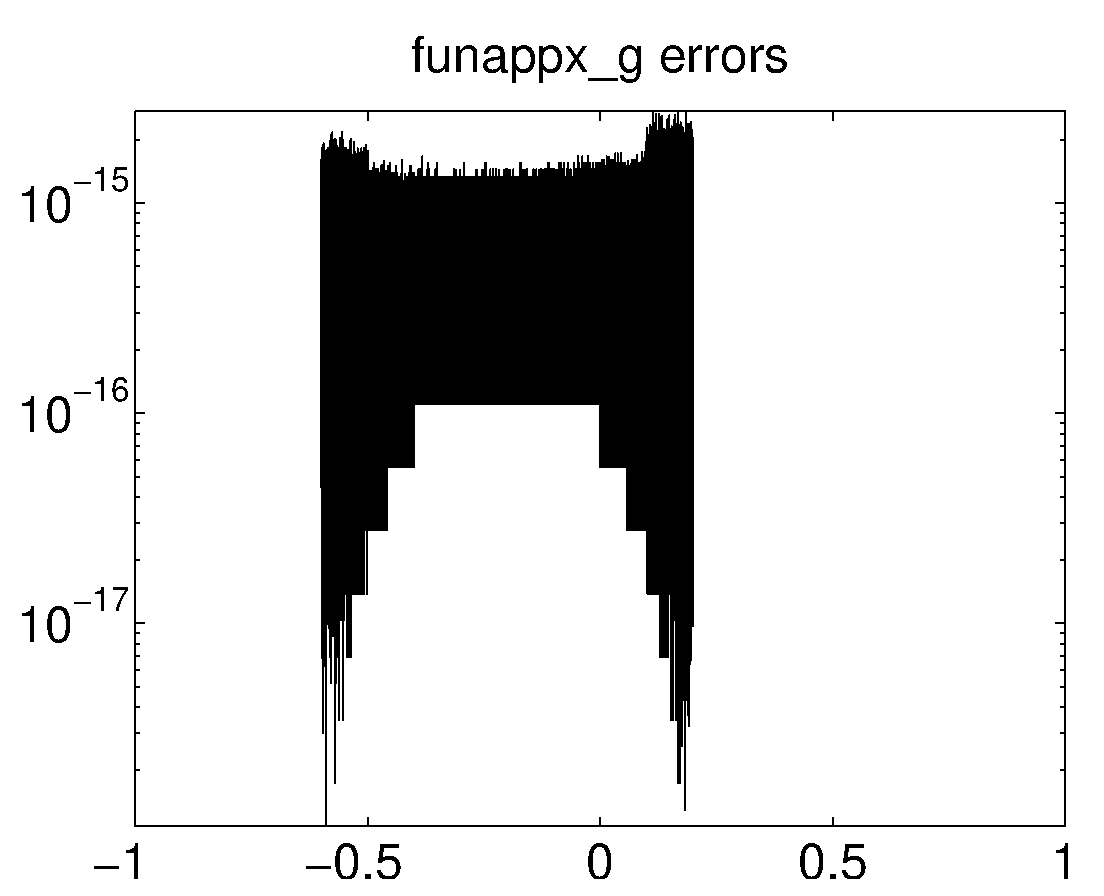
\includegraphics[width=5.9cm]{figure/funappx_g_errors.eps}
\\ a) & b)
\end{tabular}
\caption{Approximating $f_3(x)$ with errors of interpolants returned from a)
Chebfun and b) \funappxg. This figure is reproducible by
\texttt{cf\_chebfun.m}. \label{f3chebfig}}
\end{figure}
%

\end{exmp}

\begin{comment}
Our algorithm is readily extensible to the following complex-valued function.
\begin{exmp} This example is taken from MATLAB's documentation for
\texttt{interp1}. Define the complex valued function $v(x) = 5x + x^2 i$ for $x
\in [1,10]$. It is clear that the real part of $v$ is $5x$ and the imaginary
part is $x^2$. We could apply \funappxg to approximate the two parts separately.
However, it is unnecessary.
\end{exmp}
\end{comment}

%% Example 2

\begin{exmp}
In this example, we want to compare our adaptive algorithms with Chebfun by
simulating the following families of test functions in addition to $f_3$:
%
\begin{align*}
 g_1(x) &= x^4 \sin(d/x), \qquad
 g_2(x) = 10  x^2 + g_1(x),
%\\ f_3(x) &= \begin{cases} \displaystyle
%   \frac{1}{2\delta^2} \Bigl [4 \delta^2 + (x-c)^2 + (x-c-\delta)\abs{x-c-\delta}
%\\ \qquad \qquad
%    - (x-c+\delta)\abs{x-c+\delta} \Bigr ], & \abs{x-c} \le 2\delta,
%\\ 0, & \text{otherwise},
%\end{cases} \\
%\\ g_3(x) & = (x-d)^2,  \qquad
% g_4(x)= d\sin(d\pi x), \qquad
%\\ g_5(x) &= 10\exp\left(-1000(x-d)^2\right), \qquad
% \\ f_4(x)&= \frac{c}{4}\exp(-2x)(c-2\exp(x)(-1 + c\cos(x) - c\sin(x)) \\
%  & \ \ +\exp(2x)(c + 2\cos(x)- 2\sin(x) - c\sin(2x))),
\end{align*}
where $c$ for defining $f_3$ is uniformly drawn $100$ times from $[0,0.6]$ and
$d$ for other functions from $[0,2]$. If $d=1$, then  $g_i$ reduces to $f_i$ for
$i=1 \mbox{ and } 2$.
We set $\abstol = 10^{-6}$ and $\fC
(h) = \frac{ 3 \fh}{\fh-h}$ where $\fh = \frac{5(b-a)}{n_0-1}$, and we use
\texttt{funappx\_g} and \texttt{funappxglobal\_g} to approximate the test
functions on interval $[a,b]=[-1,1]$. The approximation results are
summarized in Table~\ref{tab:localVsGlobalVsChebfun}. We switch on the splitting
feature in Chebfun to use piecewise Chebyshev polynomials for approximation and override its tolerance to $10^{-6}$ as well.

%
\begin{figure}[th]
  \centering
%  \begin{tabular}{cc}
%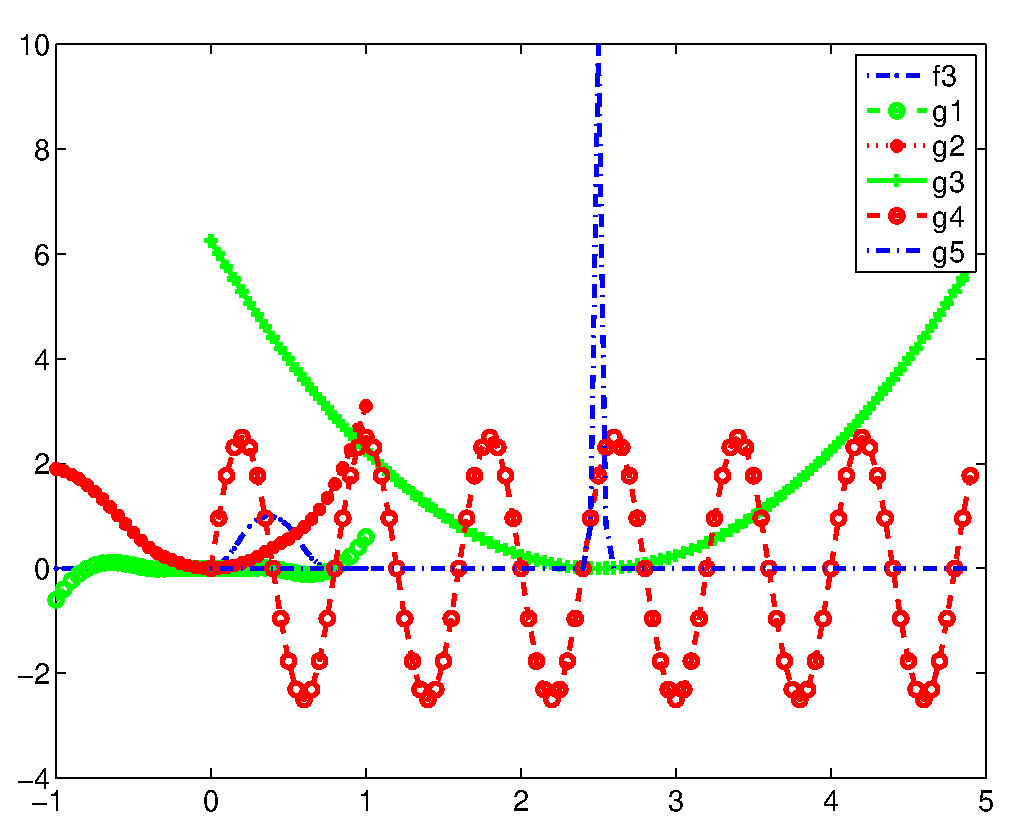
\includegraphics[width=58mm]{figure/traub_funappxNoPenalty_g_testfun.eps} & \hspace{-4ex}
\includegraphics[width=80mm]{figure/traub_funappx_g_test.eps}
%  \\ a)  & b)
%  \end{tabular}
\caption{The empirical distribution function of performance ratios based on 500 replications:  \funappxg{} time $/$ \funappxglobalg{} time (blue), \funappxg{} \# of samples $/$ \funappxglobalg{} \# of samples (orange) ,   \funappxg{} time $/$ Chebfun time (purple), \funappxg{} \# of samples $/$ Chebfun \# of samples (green). This figure is conditionally reproduced by
\texttt{traubpaper\_funappx\_g\_test.m} in GAIL.}
  \label{fig:testfunctions}
\end{figure}

%
\begin{table}[bt]
\centering
\caption{Comparison of number of sample points, computational time,  and success
rates of \funappxg, \funappxglobalg, and Chebfun.
%We also report the number of warnings in parentheses issued by the software.
This table can be conditionally reproduced by
\texttt{traubpaper\_funappx\_g\_test.m} in GAIL.}
\label{tab:localVsGlobalVsChebfun}
{\footnotesize
\setlength{\tabcolsep}{.5em} % set table width
\begin{tabular}{|c|rrr|rrr|rrrrrr|}
\hline
    Test      &     \multicolumn{3}{c|}{Mean Number of Points} & \multicolumn{3}{c|}{Mean Time Used}  & \multicolumn{6}{|c|}{Success (\%)}
\\  family &  Local  &  Global    &  Chebfun    & Local     &  Global     & Chebfun      & \multicolumn{2}{r}{Local} & \multicolumn{2}{r}{Global} & \multicolumn{2}{r|}{Chebfun}
\\ \hline
          f3   &   2904  &   46439   &   113    &   0.016   &     0.028    &   0.185 &    100   &    &  100   &   &  0   &
\\        g1   &   2996  &   27380   &    44    &   0.024   &     0.021    &   0.037 &    100   &    &  100   &   &  4   &
\\        g2   &   6926  &   97438   &    24    &   0.020   &     0.041    &   0.021 &    100   &    &  100   &   &  4   &
\\ \hline	
\end{tabular}
}
\end{table}
%

From Table~\ref{tab:localVsGlobalVsChebfun}, we see that both \funappxg{} and
\funappxglobalg{} achieved total successes---they succeeded
even for  $g_1$ outside the cone even though there are no theoretical guarantees.
The former worked better than
\funappxglobalg{} for all test cases in terms of number of sampling points and
\emph{average} run time as evidenced by Figure~\ref{fig:testfunctions}.
In contrast, Chebfun generally used substantially less number of node points
than \funappxg{} even though the run time was longer than \funappxg{} in
about~60\% of the test cases; see Figure~\ref{fig:testfunctions}.
However, it approximated satisfactorily only eight percent of the~300 test
functions.


%
\begin{table}[tbh]
	\centering
	\caption{Comparison of number of sample points, computational time,  and success
		rates of \funming, \fminbnd, and
		Chebfun's \texttt{min}.
		%We also report the number of warnings in parentheses issued by the software.
		This table can be conditionally reproduced by
		\texttt{traubpaper\_funmin\_g\_test.m} in GAIL.}
	\label{tab:funmingVsfminbndVsChebfun}
	{\footnotesize
		\setlength{\tabcolsep}{.48em} % set table width
		\begin{tabular}{|c|rrr|rrr|rrrrrr|}
			\hline
			Test      &     \multicolumn{3}{c|}{Mean Number of Points} & \multicolumn{3}{c|}{Mean Time Used}  & \multicolumn{6}{|c|}{Success (\%)}
			\\  family &  \funming  &  \fminbnd    &  \texttt{min}    & \funming     &  \fminbnd  & \texttt{min}   & \multicolumn{2}{r}{\funming} & \multicolumn{2}{r}{\fminbnd} & \multicolumn{2}{r|}{\texttt{min}}
			\\ \hline
			-f3   &  274   &   8   &   113    &   0.006   &    0.004    &  0.196  &    100   &  &  100   &   &  12 &
			\\ \phantom{-}g1   &  230   &  22   &    44    &   0.005   &    0.006    &  0.044  &    100   &  &   24   &   &  54 &
			\\ \phantom{-}g2   &  273   &   9   &    24    &   0.006   &    0.005    &  0.025  &    100   &  &  100   &   &  34 &
			\\ \hline
		\end{tabular}
	}
\end{table}
%

We conducted similar simulation test run for comparing \funming, \fminbnd, and
Chebfun's \texttt{min} and reported the results in
Table~\ref{tab:funmingVsfminbndVsChebfun}. \funming{} achieved 100\%
success rates in every case with substantially less sampling points and run time than \funappxg.
In contrast, \fminbnd{} could not locate the global
minimum at the boundary point for 76\% test functions from $g_1$, that is actually a known
limitation of the method (see documentation of the method in MATLAB). Chebfun's
{\tt min} performed better than its function approximation function but still failed in most of the cases.

\end{exmp}


\begin{comment}
\begin{exmp}
In this example, we consider the function $f_4(x) = sin(10 \pi x^4) + x$, which
is increasing oscillating over the interval $[0,2]$. We use \funappxg, \funming,
and \integralg to approximate the function, locate its global minimum, and
estimate its integral with $\abstol = 10^{-8}$. With $1,972,359$ points,
\funappxg can approximate $f_4$ uniformly accurate as shown in
Figure~\ref{f4fig}(a). The true global minimum is $(0.6212340312,
-0.3782149854)$ and the absolute approximation error of \funming using
$n=2,022,621$ points is $(1.4\times 10^{-7}, 4.7\times 10^{-11})$. The integral
$\int_{0}^{2} f_4 (x) dx = 2.145517314$ and the approximation error of
\integralg is $4.7\times10^{-10}$ using $4,965,641$ points.

\begin{figure}[bt]
\centering
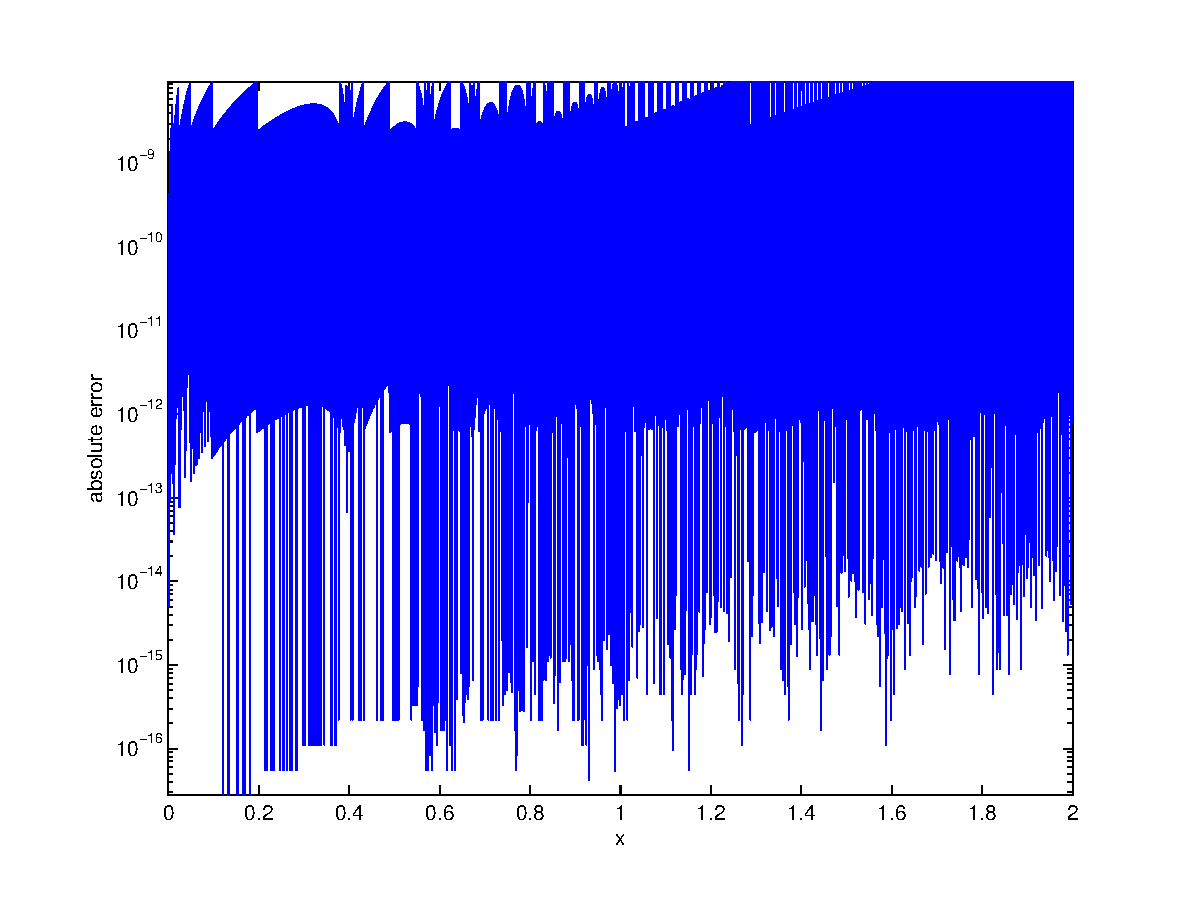
\includegraphics[width=6.2cm]{figure/f4_funappx_error.eps} \hspace{-5ex}
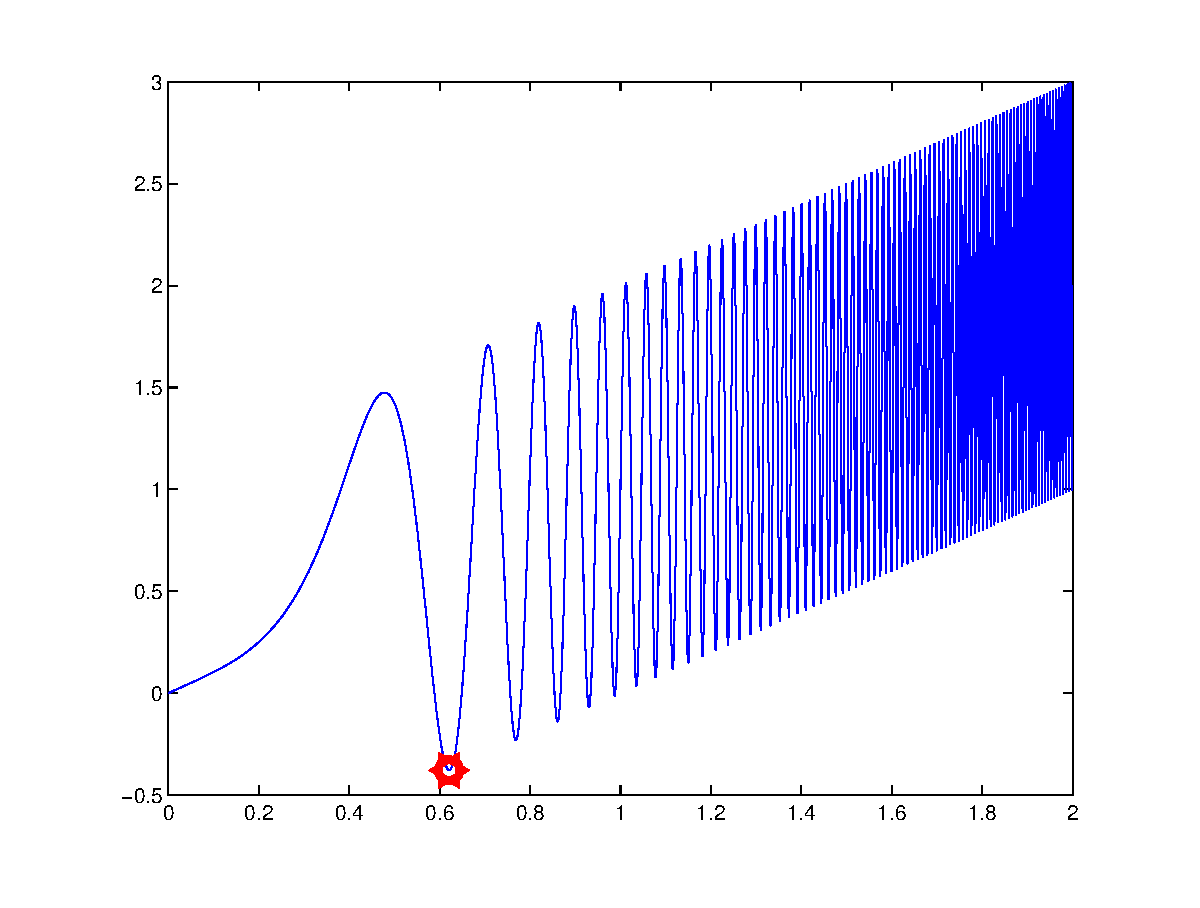
\includegraphics[width=6.2cm]{figure/f4_funmin_g.eps}
\caption{The example $f_4$ with errors of interpolants from \funappxg (left) and
minimum found by \funming (right).}
\label{f4fig}
\end{figure}
\end{exmp}
\end{comment}


\begin{comment}
Our algorithm is readily extensible to the following complex-valued function.
\begin{exmp}
This example is taken from MATLAB's documentation for \texttt{interp1}. Define
the complex valued function $v(x) = 5x + x^2 i$ for $x \in [1,10]$. It is clear
that the real part of $v$ is $5x$ and the imaginary part is $x^2$. We could
apply \funappxg to approximate the two parts separately. However, it is
unnecessary.
\end{exmp}
\end{comment}



%%%%%%%%%%%%%%%%%%%%%%%%%%%%%%%%%%%%%%%%%%%%%%%%%%
\section{Discussion}
%%%%%%%%%%%%%%%%%%%%%%%%%%%%%%%%%%%%%%%%%%%%%%%%%%

Software packages such as Chebfun and MATLAB's functions including
\texttt{interp1}, \texttt{griddedInterpolant}, and \texttt{fminbnd} are some of
the most popular and useful function interpolation and minimization methods.
However, it is important for users to be vigilant in applying these and other
similar tools, which often do not inform users of whether the approximants meet
the user's required accuracy. The reasons may range from an absence of rigorous
theoretical frameworks (e.g., no method in MATLAB's Global Optimization Toolbox
provides any certification of global solutions) for error estimation to
understandable challenges in efficient implementation.

Function approximation and minimization methods are not necessarily precise
enough unless we use a sufficiently large number of sampling points. This paper
is an effort to provide a unifying framework covering adaptive data sampling of
a given smooth and not too spiky function $f$, construction of an interpolant
$\hat{f}$, and an estimation of the corresponding maximum error bound. Our
locally adaptive strategy is to sample $f$ more frequently in subintervals where
(an upper bound of) $f''$ is large in magnitude and when the maximum error bound
over the subintervals are not meeting user-required tolerance. Hence a novelty
of our algorithms is its capability to choose a suitable granularity of distinct
data points $\{(x_i, f(x_i))\}_{i=1}^n$ in order to warrant that the
interpolation error satisfies user-given tolerance, that is $\| f - \hat{f} \|
\le \abstol$.

We have implemented our algorithms in a MATLAB toolbox we call
GAIL~\cite{ChoEtal15a}. As a side note, the package is under active development
guided by the latest theoretical developments of cones of functions and
constructed according to our best knowledge of good practices of MATLAB
programming, which include interfaces for input parsing, doc tests and unit
tests, as well as code comments and searchable HTML user guide and
documentation.

In the rest of this section, we would like to suggest some future work areas.

Our approach is not necessarily fast for all functions $f$ or in high precision
setting as we are simply using linear splines. However, it is embarrassingly
easy to parallelize our algorithms by using MATLAB's Parallel Computing Toolbox
on a modern multicore machine and applying our methods to each subinterval in a
contiguous partition of the domain followed by some simple post processing.

Our linear interpolants are not smooth and may require a sizable number of data
points for tiny tolerance or spiky functions. For future work, better choices of
basis functions for coming up with a function approximant are important for
enhancing smoothness and data efficiency. Cubic splines, radial basis functions,
and Chebyshev polynomials are some potential promising candidates.

We can also consider developing guaranteed adaptive algorithms for high
dimensional functional approximation and optimization. For $d=2$, we can
construct a triangular or rectangular mesh, and refine the mesh until we reach
given error tolerance. More generally, some relevant ideas are contained in the
recent work of Zhou and Hickernell for multidimensional-function approximation
using radial basis functions~\cite{ZhoHic15a}---unfortunately, the associated
error bounds are too restrictive in the sense that they are applicable only to
tiny domains, and consequently have not made a practical impact.

Our algorithms provides guaranteed accuracy based on absolute error tolerance.
This analysis could be extended to include \emph{relative} error tolerance
$\varepsilon_r$, for example, $ \| f -\hat{f} \|_{\infty} \le \max{
\{\varepsilon, \varepsilon_r \norm[\infty]{f} \} }.$ Even though
$\norm[\infty]{f}$ is unknown, it can be estimated at increasing accuracy from
the data points iteratively.

One may consider our global minimization algorithm an application of our
function approximation method. Likewise, it is foreseeable that
similarly robust and efficient algorithms such as root finding or
numerical solutions of differential equations could be built upon our framework.


\section*{Acknowledgements}
We dedicate this paper to the memory of our colleague Joseph F. Traub, who
passed away on August 24, 2015. He was a polymath and an influential figure in
computer science and applied mathematics. He was the founding Editor-in-Chief of
the Journal of Complexity and we are grateful to his tremendous impact and life
long services to our research community.

We would like to thank our colleagues Greg Fasshauer and the GAIL team
for valuable suggestions and comments. This research was supported in part by
grant NSF-DMS-1522687.



%%%%%%%%%%%%%%%%%%%%%%%%%%%%%%%%%%%%%%%%%%%%%%%%%%
%\section*{References}
%%%%%%%%%%%%%%%%%%%%%%%%%%%%%%%%%%%%%%%%%%%%%%%%%%

\bibliography{FJH23,FJHOwn23}

\end{document}








